\documentclass[12pt,a4paper]{ctexart}

\usepackage{amsmath,amssymb}
\usepackage{graphicx}
\usepackage{float}
\usepackage{geometry}
\usepackage{hyperref}
\usepackage{booktabs}
\usepackage{array}
\usepackage{caption}
\usepackage{subcaption}
\usepackage{enumitem}
\usepackage{fancyhdr}
\usepackage{xcolor}
\usepackage{tabularx}
\usepackage{listings}

\geometry{left=2.5cm,right=2.5cm,top=2.5cm,bottom=2.5cm}
\graphicspath{{./}{act_figures/}}
\hypersetup{colorlinks=true,linkcolor=blue,urlcolor=blue,citecolor=blue}
\setlength{\headheight}{15pt}
\renewcommand{\arraystretch}{1.15}
\setlist[itemize]{itemsep=2pt,topsep=3pt}
\setlist[enumerate]{itemsep=2pt,topsep=3pt}
\lstset{
    basicstyle=\ttfamily\small,
    frame=single,
    breaklines=true,
    columns=fullflexible
}

\pagestyle{fancy}
\fancyhf{}
\fancyhead[L]{深度学习与空间智能——实验报告}
\fancyhead[R]{期末作业：题目一与题目二}
\fancyfoot[C]{\thepage}

\begin{document}

\begin{titlepage}
    \centering
    \vspace*{2.2cm}
    {\zihao{1}\bfseries 深度学习与空间智能期末作业报告\par}
    \vspace{1.8cm}
    \begin{tabular}{>{\bfseries}p{3.0cm}p{10.5cm}}
        小组成员 & 李响 25210980071；张博宇 25210980133 \\
        分工说明 & 张博宇负责题目一：基于 3DGS 与 AIGC 的多源资产生成与真实场景融合；李响负责题目二：基于 LeRobot 的 ACT 策略跨环境泛化挑战。\\
    \end{tabular}
\end{titlepage}

\tableofcontents
\newpage

\section{整体说明}

本报告整合两个作业方向。第一部分面向 3D 视觉资产生成与融合，覆盖真实多视角重建、文本到 3D、单图到 3D、背景场景重建和最终场景融合渲染；第二部分面向具身智能策略学习，基于 LeRobot 框架训练 ACT（Action Chunking with Transformers）策略，并比较环境 A 单域训练与 A+B+C 多域训练在未见环境 D 上的 zero-shot 泛化表现。

两部分分别对应作业题目一与题目二，但报告组织上尽量保持统一：每个实验均说明任务目标、方法流程、关键设置、结果现象、失败原因与改进方向。代码仓库与模型权重链接见补充材料。

\section{题目一：基于 3DGS 与 AIGC 的多源资产生成与真实场景融合}

% ==================== 一、物体A：多视角重建——扑克牌 ====================
\subsection{物体A：真实多视角重建——扑克牌}

使用手机拍摄扑克牌的环绕视频，采用\textbf{COLMAP + 3DGS}管线：COLMAP提取SIFT特征进行SfM稀疏重建获得相机位姿，再以3DGS进行可微渲染优化，学习高斯球的位置、协方差、颜色与不透明度参数，最后导出PLY格式，再手动把ply文件转化成obj文件。

\begin{figure}[H]
    \centering
    \begin{subfigure}[b]{0.48\textwidth}
        \centering
        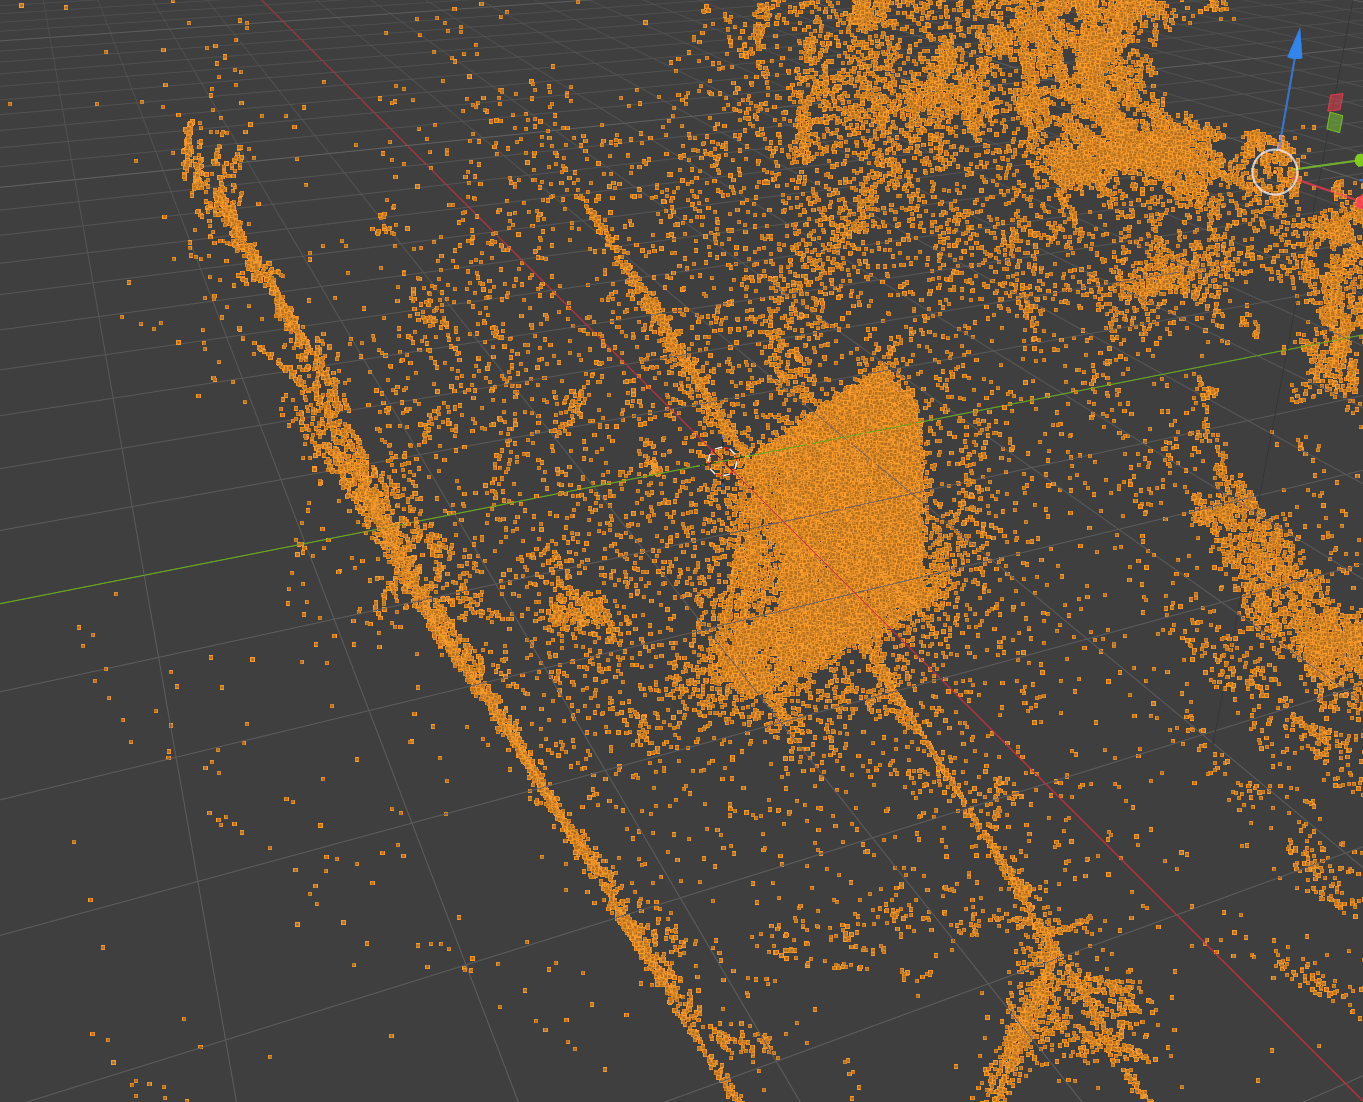
\includegraphics[width=\textwidth]{扑克牌ply文件.png}
        \caption{扑克牌PLY点云}
    \end{subfigure}
    \hfill
    \begin{subfigure}[b]{0.48\textwidth}
        \centering
        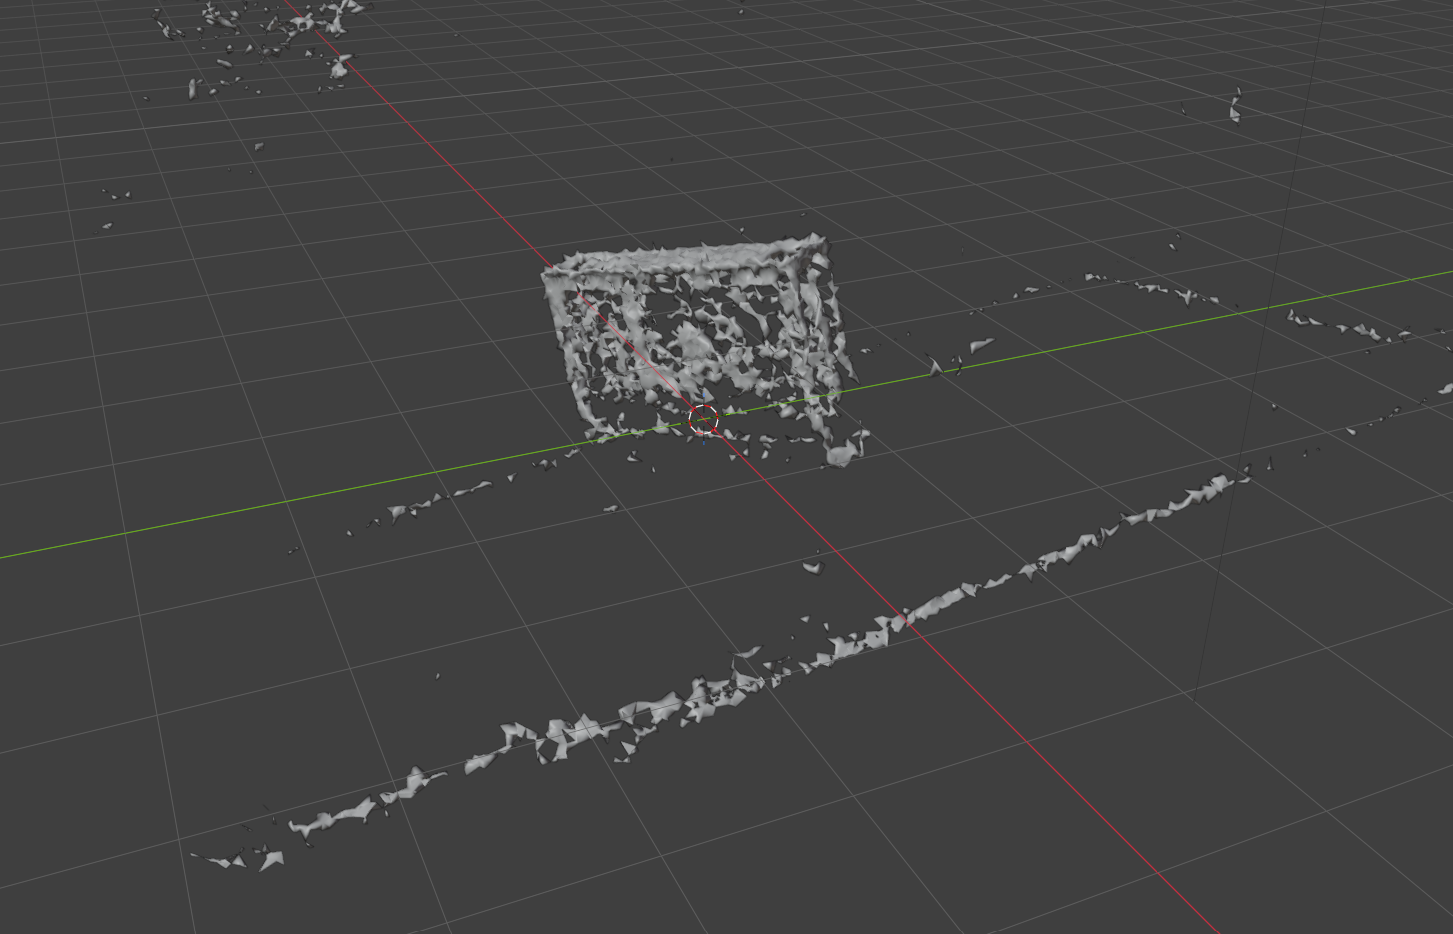
\includegraphics[width=\textwidth]{扑克牌obj文件.png}
        \caption{扑克牌OBJ模型}
    \end{subfigure}
    \caption{物体A——扑克牌的多视角重建结果}
\end{figure}

3DGS一定程度上成功重建了扑克牌的几何形态，但是生成的物体把地砖的缝隙也作为扑克牌的一部分提取进去了，而且由于手动拍摄环绕视频很难避免出现影子，模型将影子也作为物体的一部分给提取进去了，生成的点云能看出地砖的缝隙和物体轮廓，以及一些阴影导致的噪声点。

\textbf{计算耗时：}COLMAP稀疏重建约15分钟，3DGS训练约30分钟，模型导出约5分钟。

% ==================== 三、物体B：文本到3D生成——黑色无线鼠标 ====================
\subsection{物体B：文本到3D生成——黑色无线鼠标}

使用\textbf{threestudio}框架，基于Stable Diffusion与SDS Loss，通过文本Prompt \textit{``a black wireless computer mouse''} 生成3D模型。SDS Loss将渲染的2D图像送入预训练扩散模型，利用其先验知识指导3D参数优化。

\begin{figure}[H]
    \centering
    \begin{subfigure}[b]{0.48\textwidth}
        \centering
        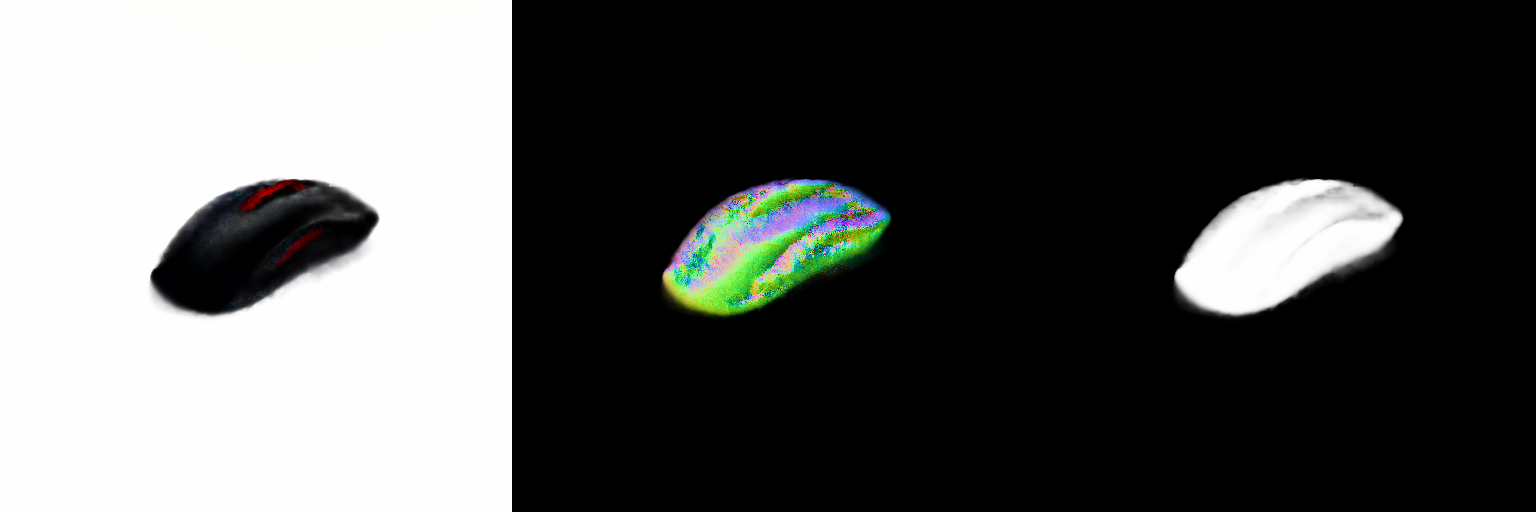
\includegraphics[width=\textwidth]{鼠标三视图.png}
        \caption{鼠标三视图}
    \end{subfigure}
    \hfill
    \begin{subfigure}[b]{0.48\textwidth}
        \centering
        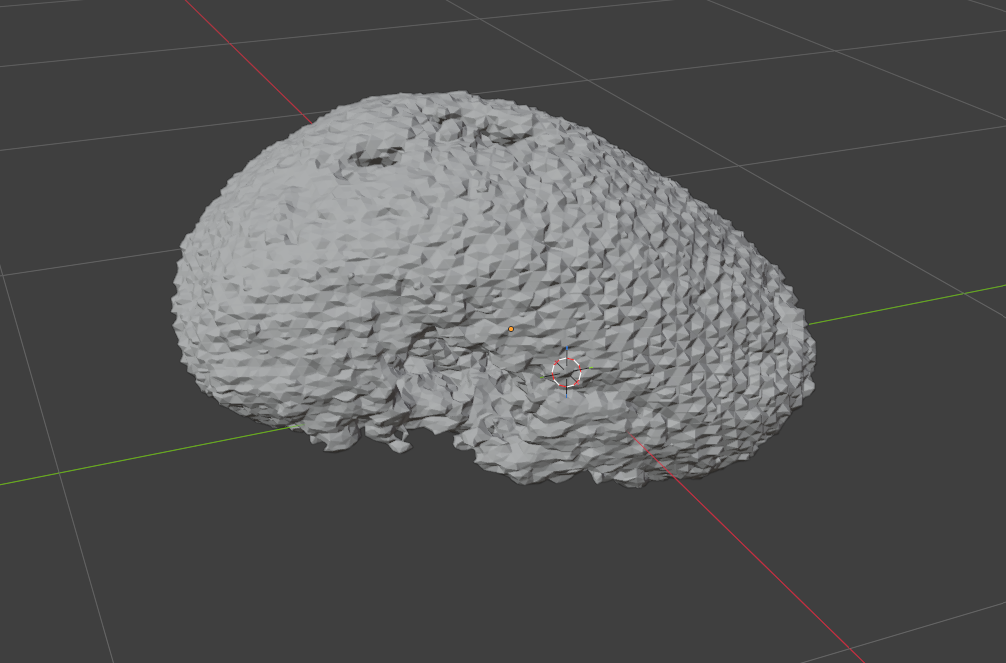
\includegraphics[width=\textwidth]{鼠标obj文件.png}
        \caption{鼠标OBJ模型}
    \end{subfigure}
    \caption{物体B——黑色无线鼠标的文本到3D生成结果}
\end{figure}

threestudio生成了鼠标的整体轮廓和曲面造型，基本符合鼠标的外观特征。但受SDS Loss模糊性影响，纹理细节偏抽象，滚轮和按键的几何边界直接呈现塌陷状。

\textbf{计算耗时：}threestudio训练1小时，模型导出约10分钟。

% ==================== 四、物体C：单图到3D生成——充电插头 ====================
\subsection{物体C：单图到3D生成——充电插头}

使用手机拍摄充电插头照片，去除背景获得纯净前景，再通过\textbf{Stable Zero123}生成新视角图像作为监督，在threestudio中优化3D隐式表示并导出OBJ。

\begin{figure}[H]
    \centering
    \begin{subfigure}[b]{0.48\textwidth}
        \centering
        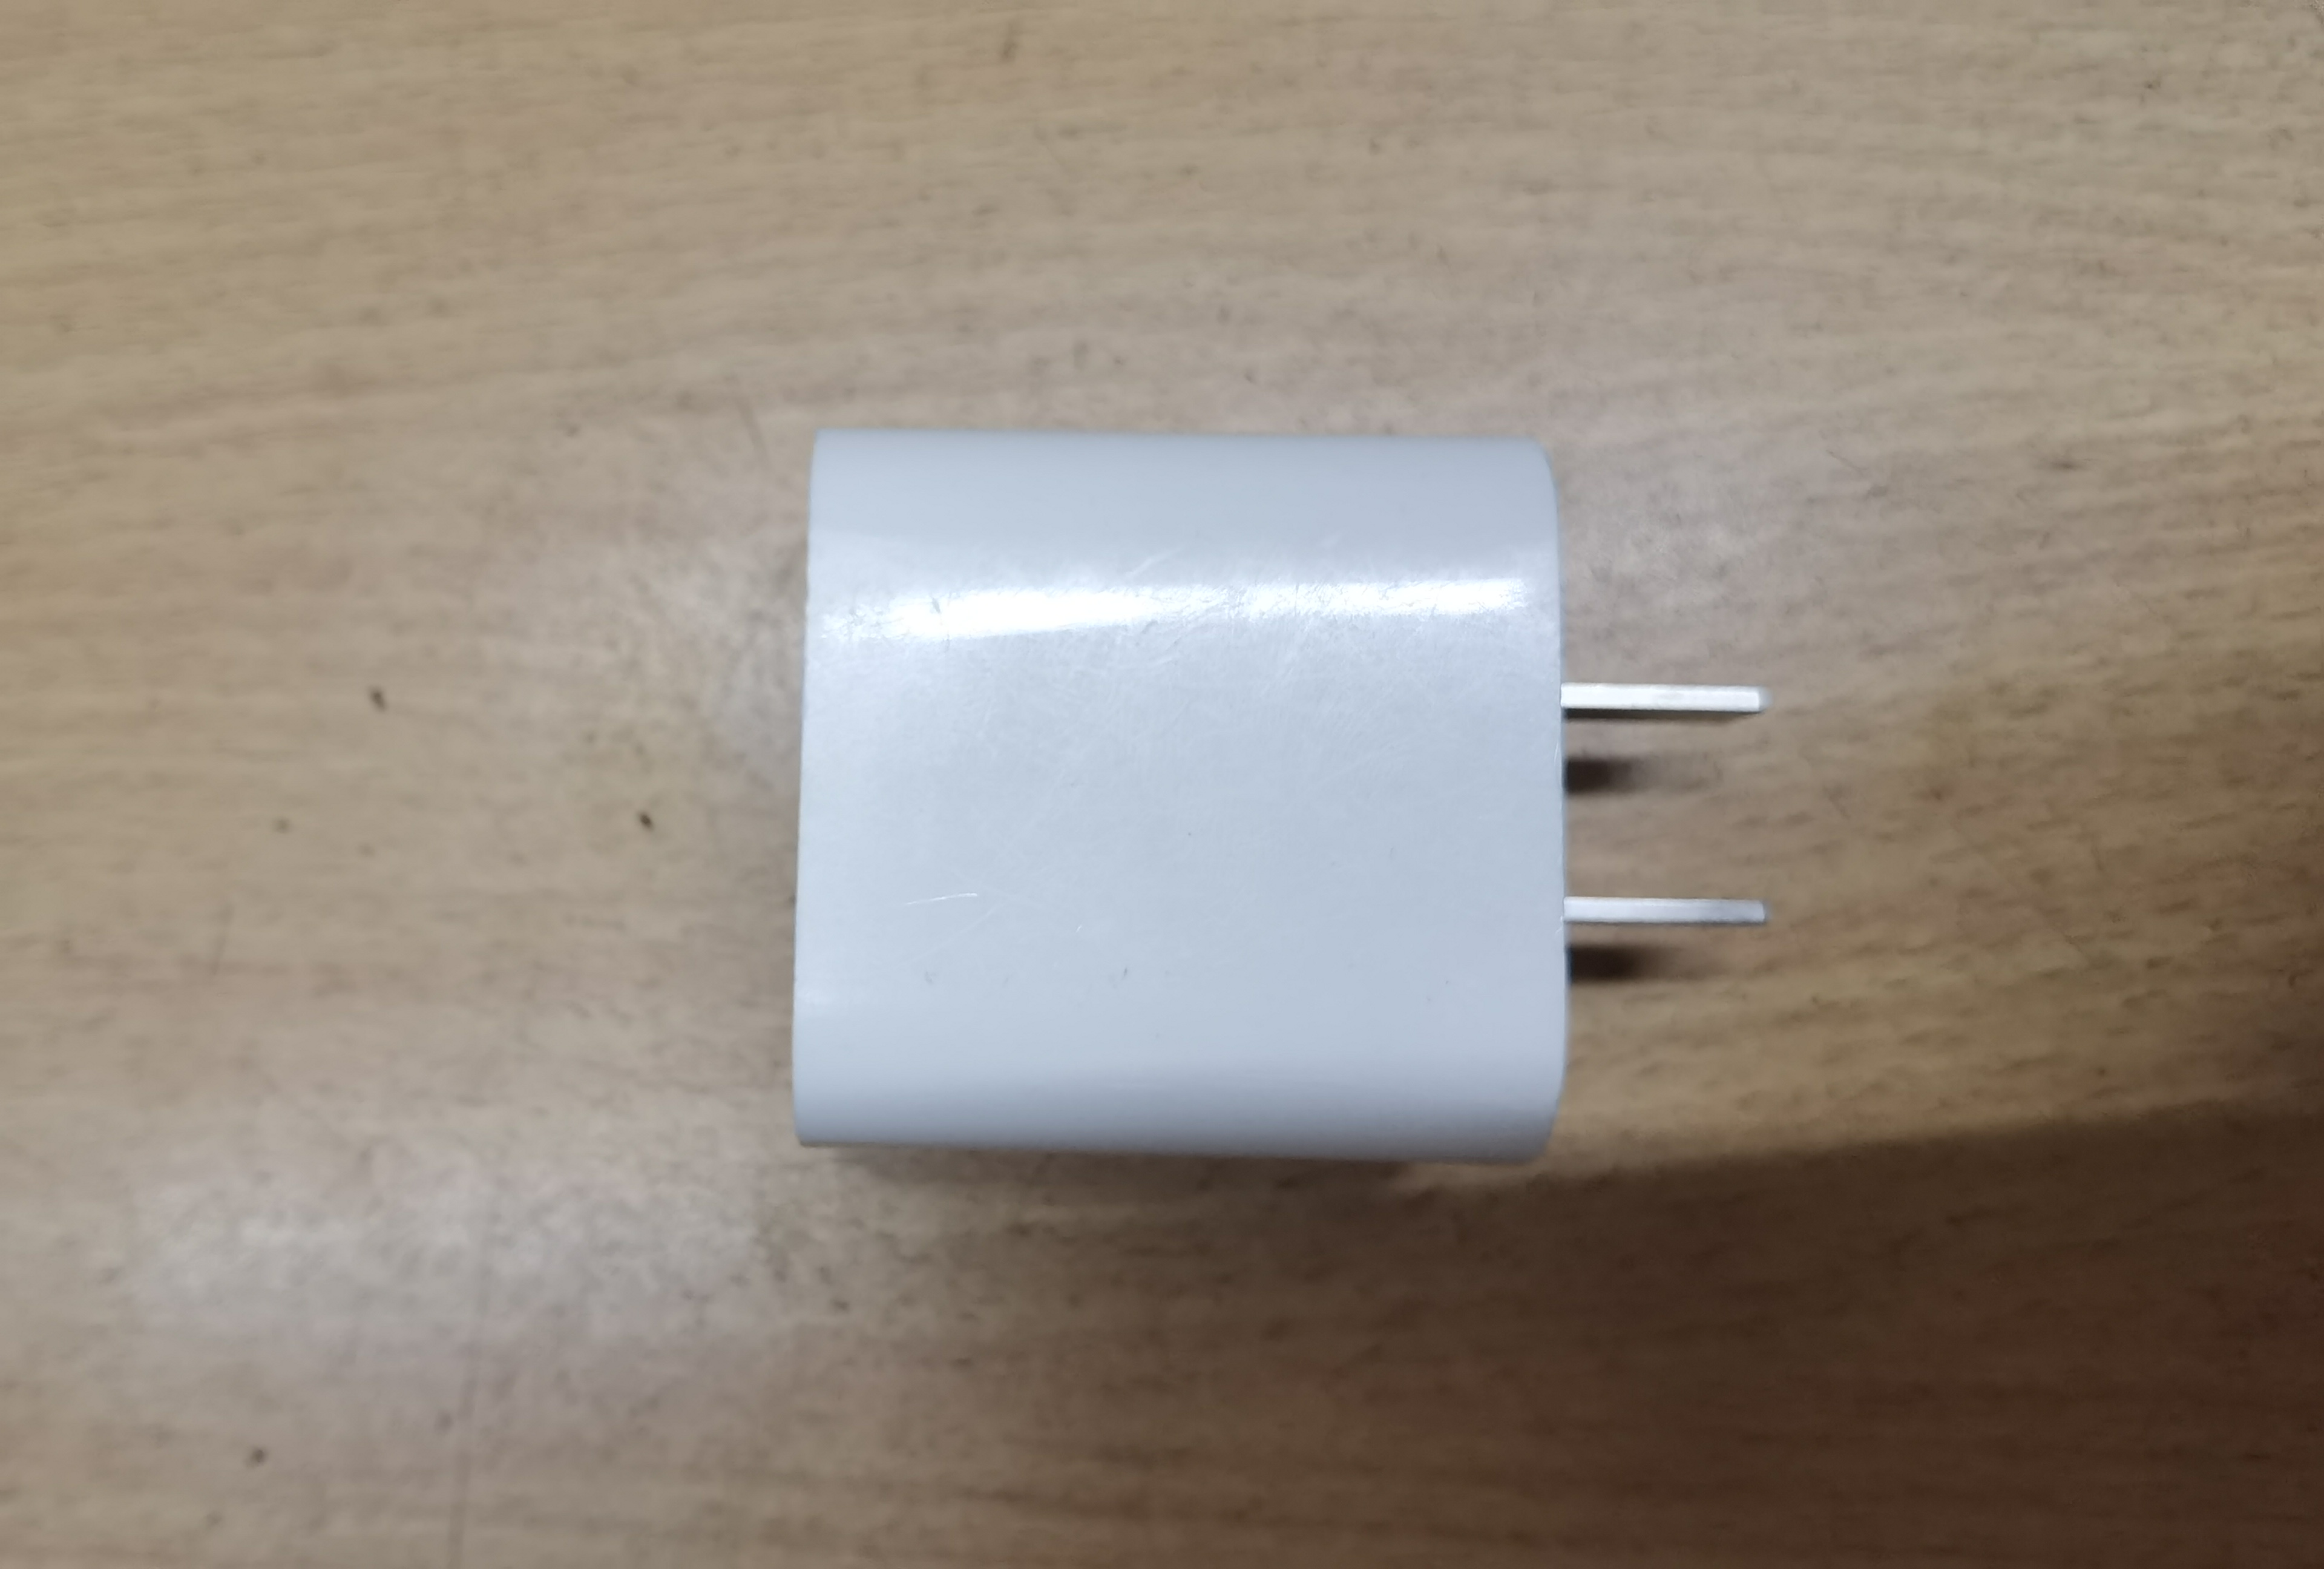
\includegraphics[width=\textwidth]{充电插头.jpg}
        \caption{原始拍摄照片}
    \end{subfigure}
    \hfill
    \begin{subfigure}[b]{0.48\textwidth}
        \centering
        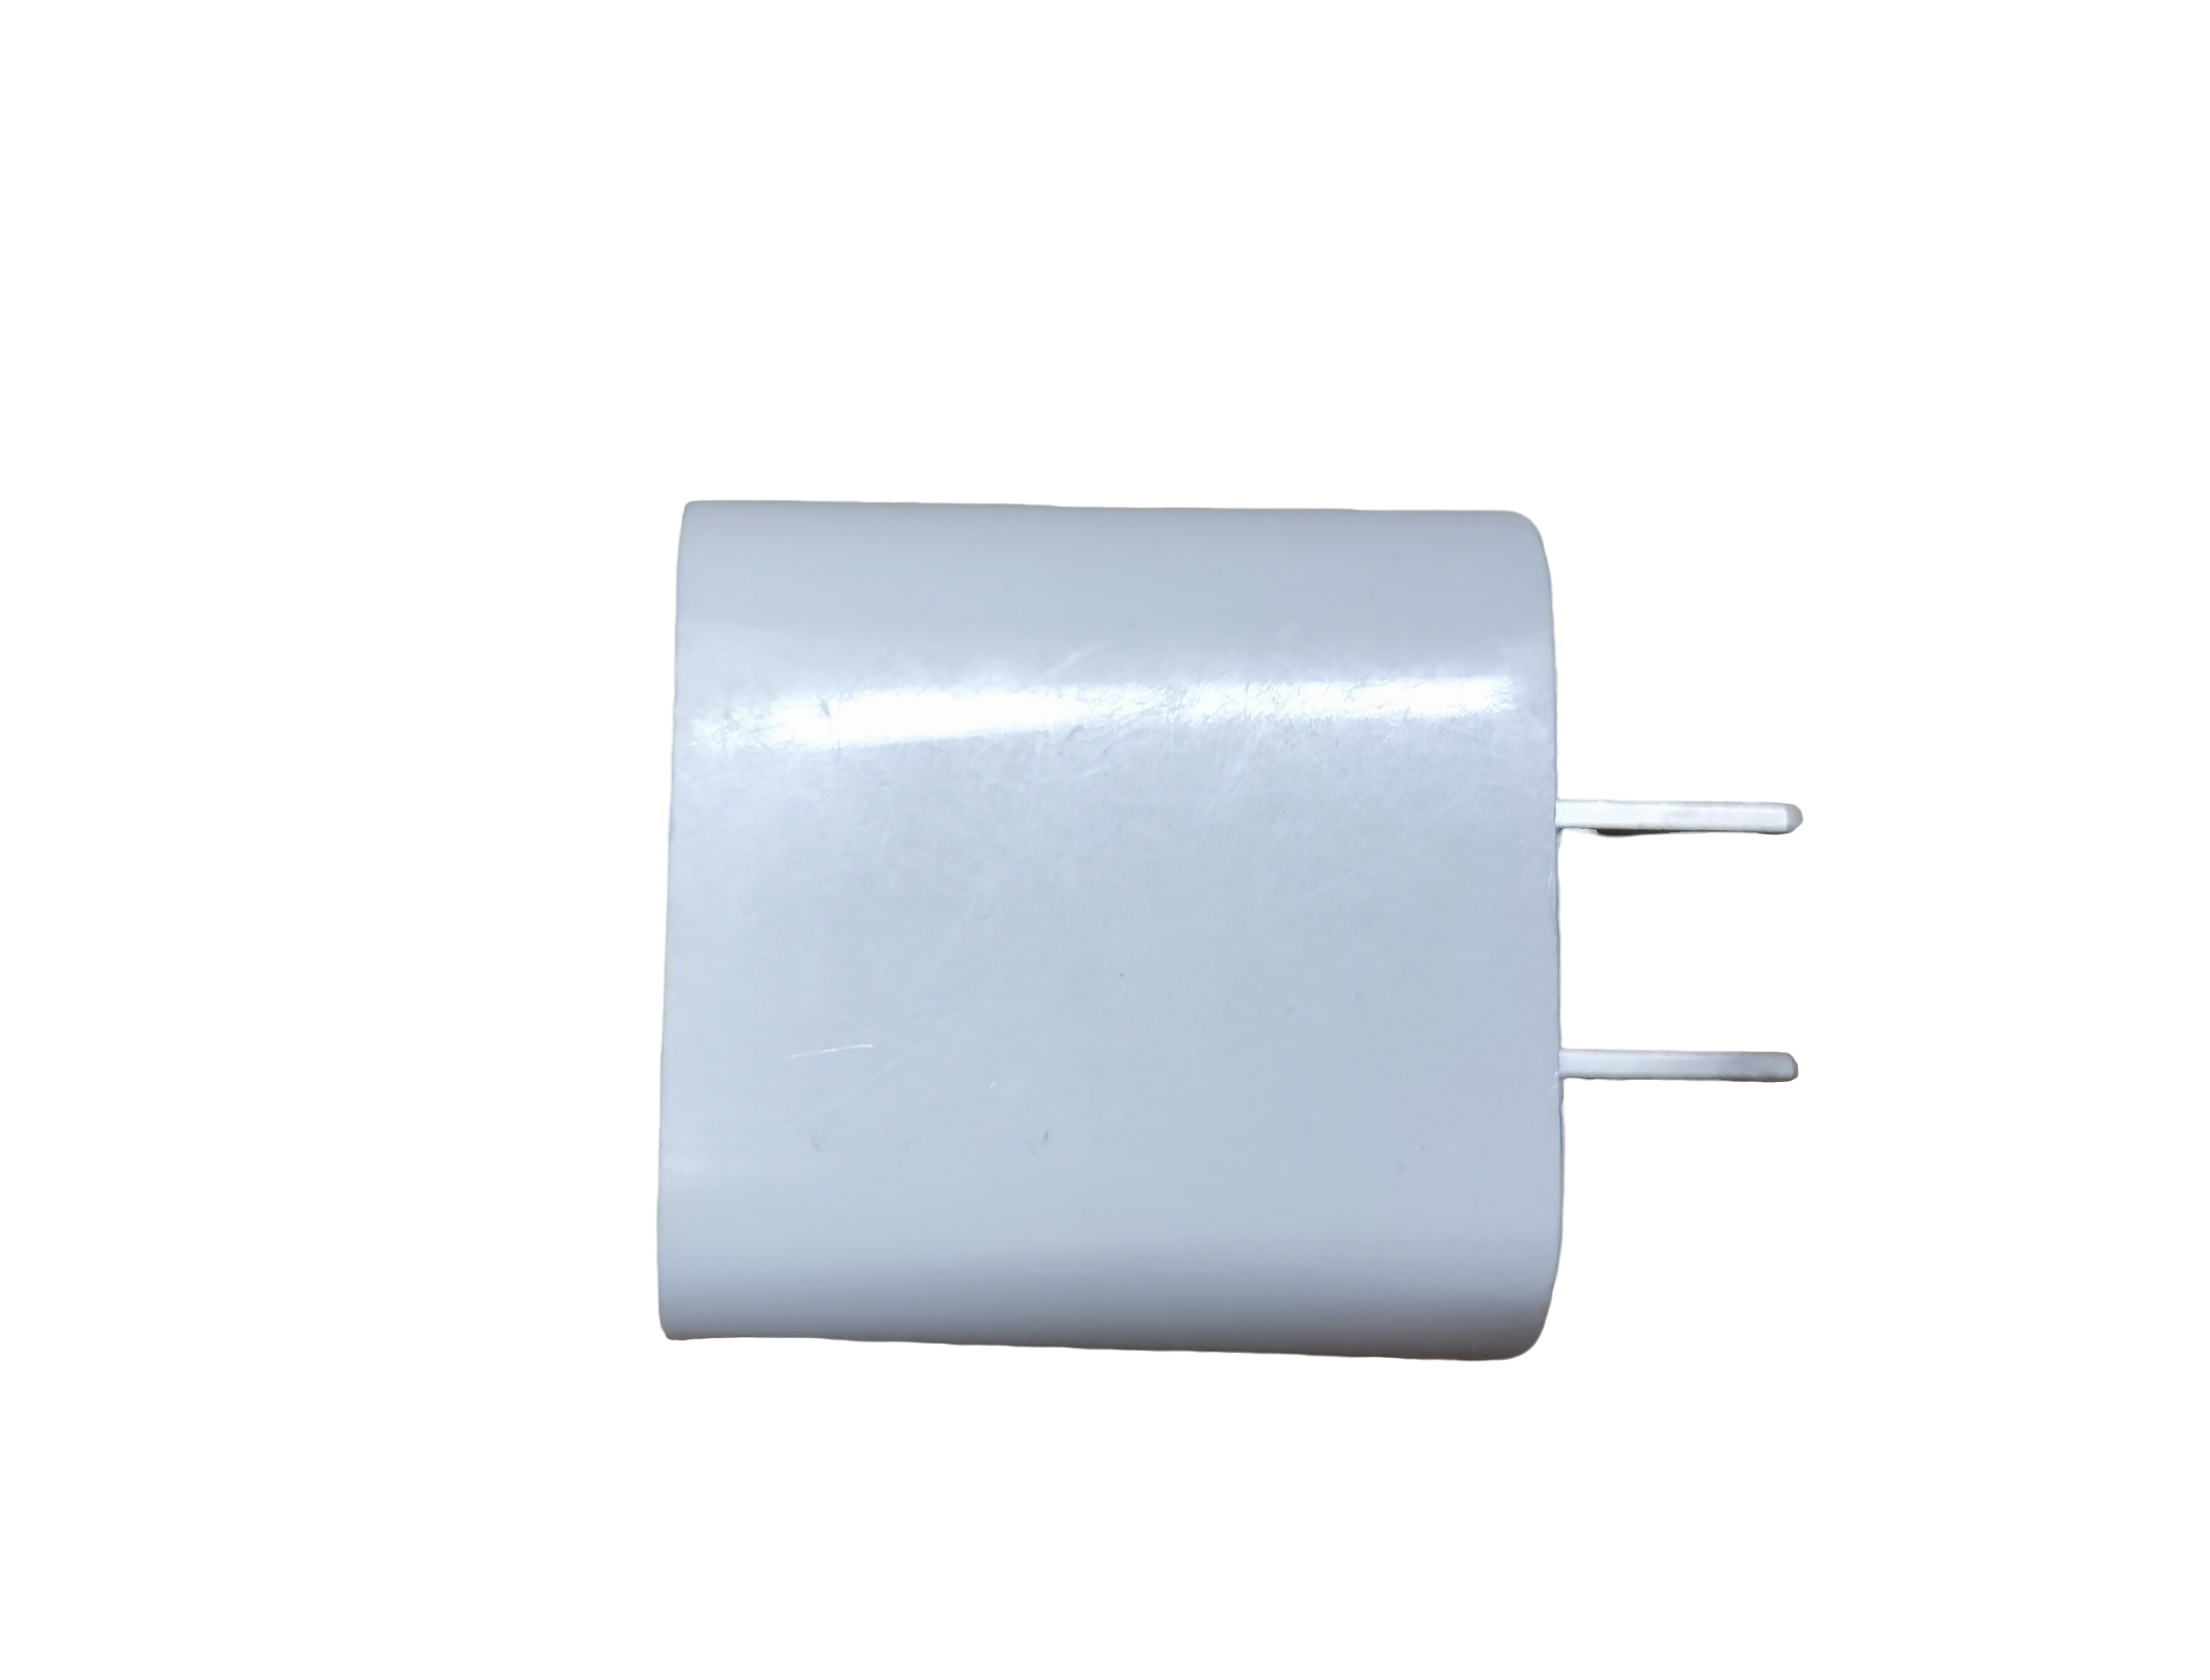
\includegraphics[width=\textwidth]{充电插头去除背景.png}
        \caption{去除背景后}
    \end{subfigure}
    \caption{物体C——充电插头的数据预处理}
\end{figure}

\begin{figure}[H]
    \centering
    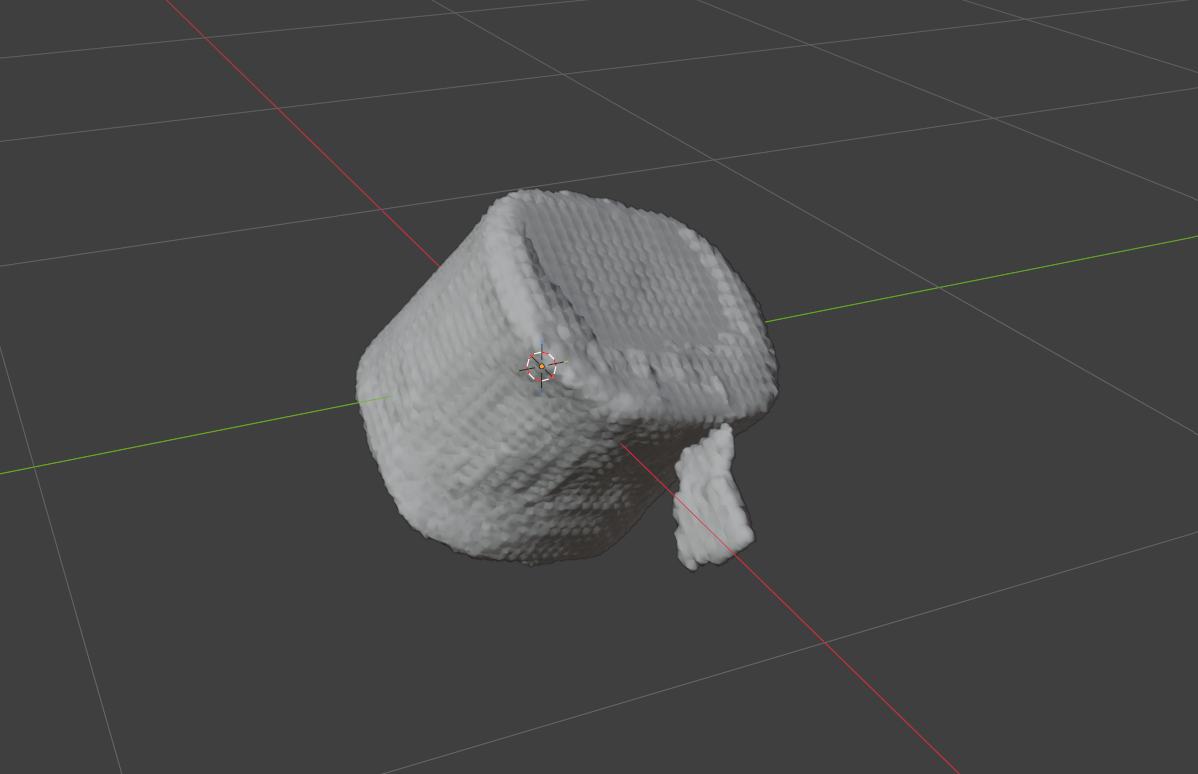
\includegraphics[width=0.6\textwidth]{充电插头obj文件.png}
    \caption{物体C——充电插头OBJ模型}
\end{figure}

几何形状基本还原了原物体结构（主体和金属引脚），纹理接近原图，但金属引脚和主题部分没有连接，被识别为了两个物体，并且两个引脚只生成了一个。

\textbf{计算耗时：}Zero123生成约20分钟，threestudio优化约1小时。

% ==================== 五、背景场景重建 ====================
\subsection{背景场景重建——Garden}

从Mip-NeRF 360数据集中选择garden场景，使用3DGS进行迭代训练重建。

\begin{figure}[H]
    \centering
    \begin{subfigure}[b]{0.48\textwidth}
        \centering
        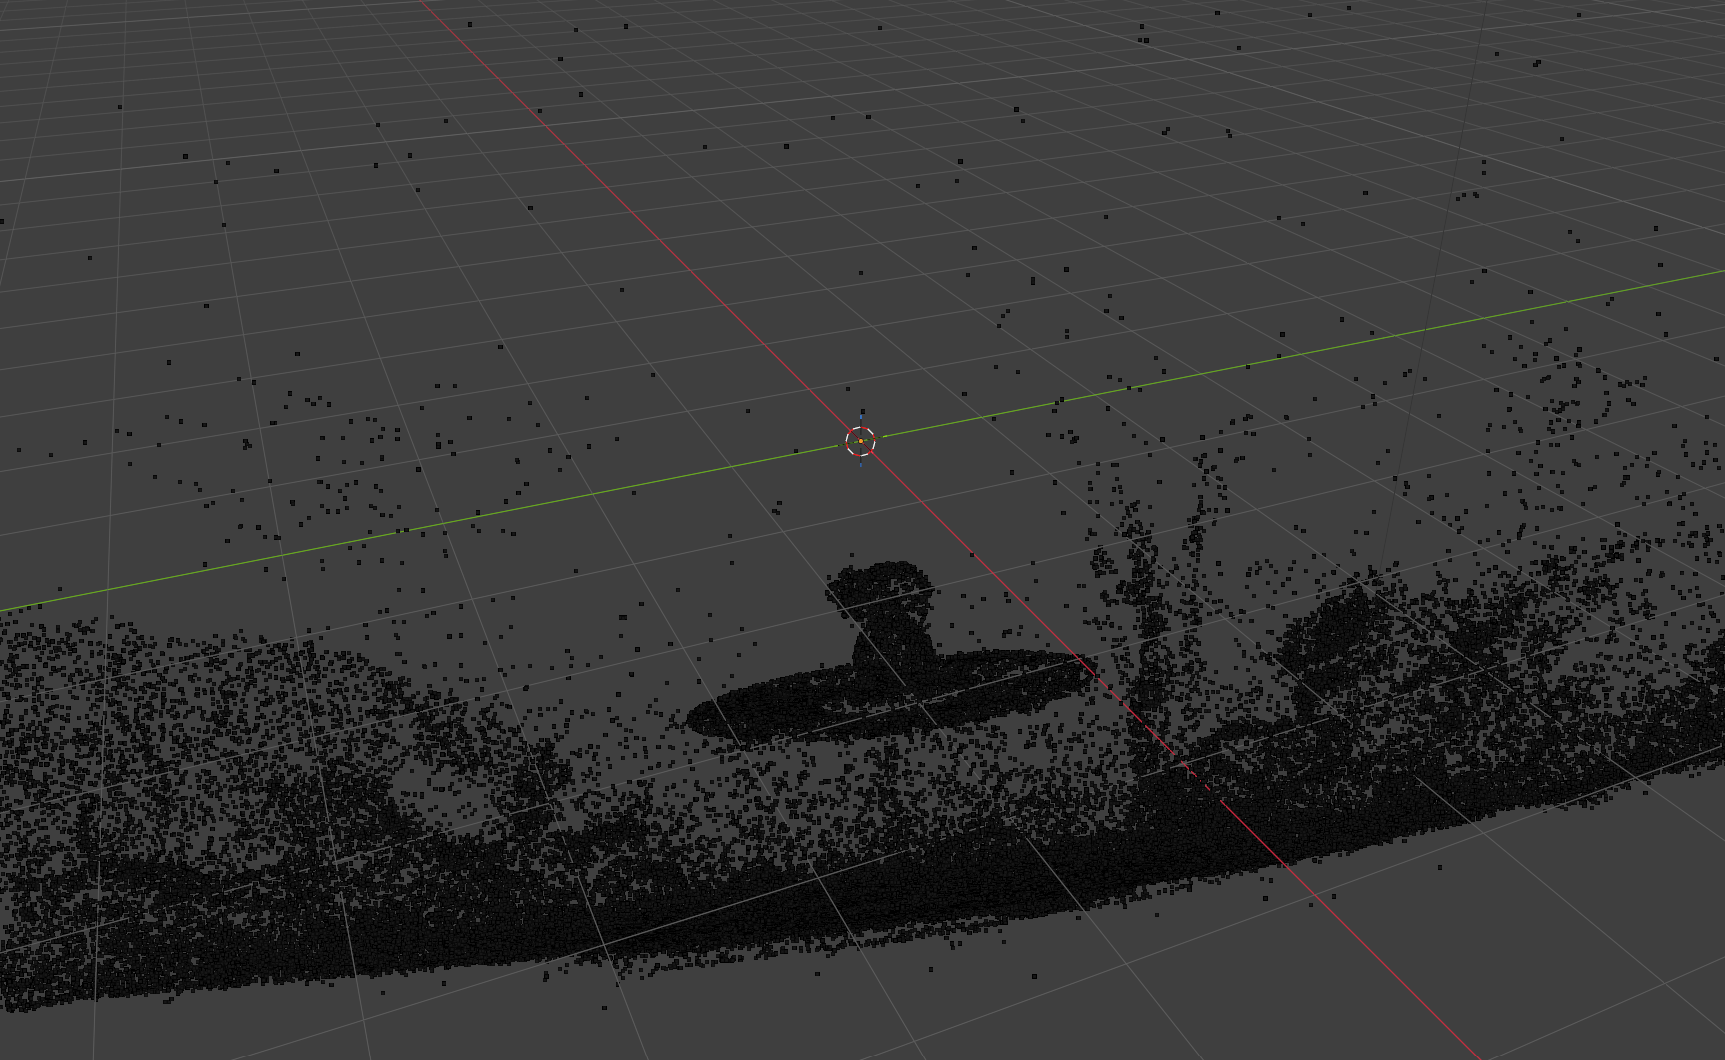
\includegraphics[width=\textwidth]{garden_ply文件.png}
        \caption{Garden PLY点云}
    \end{subfigure}
    \hfill
    \begin{subfigure}[b]{0.48\textwidth}
        \centering
        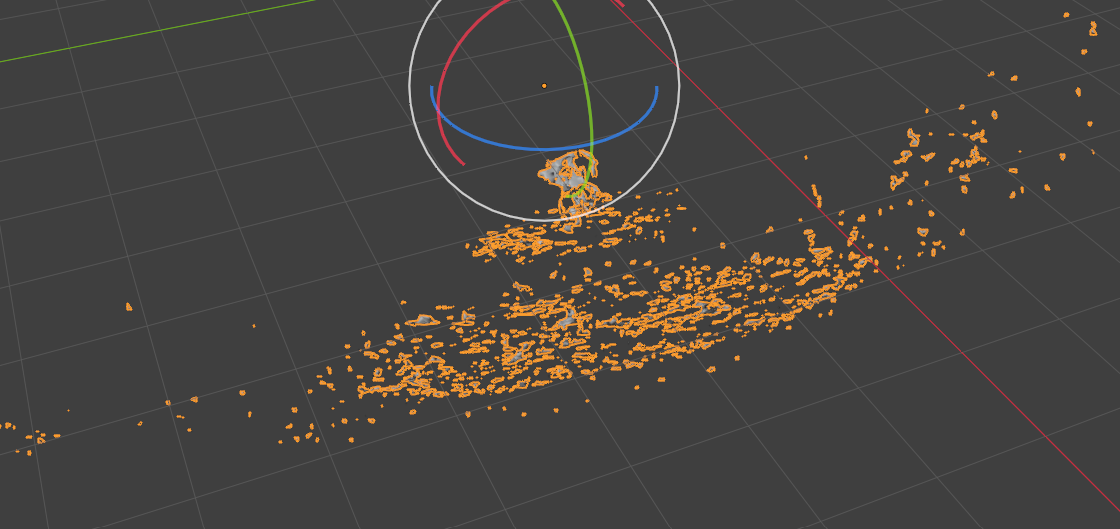
\includegraphics[width=\textwidth]{garden的obj文件.png}
        \caption{Garden OBJ模型}
    \end{subfigure}
    \caption{背景场景——Garden的3DGS重建结果}
\end{figure}

花园中的植被、步道、建筑结构并未被良好重建，只有若干拥有明确几何边界的物体能够被清晰的辨识出来。

\textbf{计算耗时：}3DGS训练50分钟。

% ==================== 六、场景融合与渲染 ====================
\subsection{场景融合与渲染}

\subsubsection{各物体重建效果总结}

三种技术路径均完成了3D模型的生成，但受限于多方面因素，重建精度有限：

\textbf{物体A（扑克牌，多视角重建）：}理论上多视角重建应获得最优几何精度，但实际效果并不理想。原因主要有两方面：一是手机手持拍摄的环绕视频不够稳定，视角覆盖不够密集，导致COLMAP的SfM位姿估计精度不足；二是拍摄时无法避免地面纹理和物体阴影进入画面，3DGS将这些背景元素也作为物体的一部分进行了重建，导出的PLY点云中夹杂了大量来自地砖缝隙和阴影的噪声点。

\textbf{物体B（鼠标，文本到3D）：}threestudio基于SDS Loss的生成方式仅依赖语义级监督，缺乏对几何细节的精确约束。同时受限于算力，训练迭代次数和分辨率均受到限制，导致鼠标的滚轮和按键等精细结构出现几何塌陷，纹理也偏模糊抽象。

\textbf{物体C（充电插头，单图到3D）：}单张照片提供的3D信息天然不完整，Zero123对不可见面的推断存在不确定性。实际生成结果中，充电插头的金属引脚与主体未能正确连接，被识别为两个独立部分，且两个引脚只生成出一个，暴露出单图到3D方法在遮挡区域几何推理上的不足。

\textbf{背景Garden：}garden为户外大场景，原始图像分辨率高、视角多，对显存需求极大。在低显存下训练，不得不降低分辨率和高斯球数量上限，导致仅具有明确几何边界的物体（如建筑结构）能被辨识，植被等细节丰富的区域重建质量有限。

\subsubsection{融合方案}

将所有模型统一转换为OBJ格式后导入Blender，按实际比例调整三者的尺寸与空间位置，设置统一光照环境，使用Cycles渲染器生成多视角漫游视频（鼠标充电插头扑克牌garden.mp4），相机环绕场景平滑移动。由于各模型本身的质量限制，融合效果受到一定影响，但本实验基本完成了从数据采集、3D生成、背景重建到场景融合的全链路流程验证。

\clearpage
\section{题目二：基于 LeRobot 的 ACT 策略跨环境泛化挑战}

\subsection{实验目的}

本实验旨在考察 ACT（Action Chunking with Transformers）策略在 CALVIN 不同视觉环境之间的跨域泛化能力。具体而言，实验在 Hugging Face LeRobot 框架下构建两个对照模型：一个仅使用环境 A 的示教数据训练，另一个使用环境 A、B、C 合并后的多环境数据训练；随后在训练过程中完全未见过的环境 D 上进行 zero-shot action prediction 测试，并以归一化 action 空间中的 L1 误差作为主要评价指标。

本部分工作完成了 CALVIN 数据集的 LeRobot 格式整理、特征键名归一化、A+B+C 多环境数据集合并、两组 ACT 模型训练、环境 D 离线评估以及训练曲线和误差分布可视化。由于本地实验没有接入 CALVIN 官方仿真 rollout，本报告未统计官方 Success Rate，而将 held-out 环境 D 上的 Action L1 作为可复现的离线泛化指标，并在讨论中说明该替代指标的局限。

\subsection{方法背景}

机器人模仿学习（Imitation Learning）从示教轨迹 $\tau=\{(o_t,a_t)\}$ 中学习策略 $\pi(a|o)$，目标是在给定视觉观测和机器人状态时预测接近专家示教的动作。与强化学习不同，模仿学习可以直接利用离线示教数据训练，适合 CALVIN 这类桌面操作任务。

ACT（Action Chunking with Transformers）不是只预测单步动作，而是一次预测未来一段动作序列，即 action chunk。本实验中 chunk size 为 100，表示模型在当前双相机图像和机器人状态输入下输出未来 100 步动作。ACT 的优势是可以利用短期时序结构，使动作序列更平滑；缺点是如果部署时长时间开环执行，后段动作可能累积误差，因此本实验额外做了 chunk horizon 分析。

CALVIN 数据集将桌面环境分为 A、B、C、D 四个视觉域，不同环境存在背景纹理、光照、物体布局等差异。本实验使用 A 或 A+B+C 作为训练域，在 D 上测试，即典型的 domain generalization 设置。直觉上，多环境训练可能学习更稳定的视觉表征；但在训练步数较短时，多域数据也会增加拟合难度，因此需要通过实验验证。

\subsection{数据集与预处理}

本实验使用 CALVIN 的 LeRobot 格式子集。A、B、C 为训练可见环境，D 为训练未见环境。为保证两个模型公平对照，只改变训练数据来源，保持网络结构和训练超参数一致。

\begin{table}[H]
    \centering
    \caption{CALVIN split 规模与实验角色}
    \begin{tabular}{llrrrr}
        \toprule
        Split & 实验角色 & Episodes & Frames & FPS & Tasks \\
        \midrule
        A & 单环境训练 baseline & 6089 & 366693 & 10 & 389 \\
        B & 多环境训练组成部分 & 6115 & 367096 & 10 & 389 \\
        C & 多环境训练组成部分 & 5666 & 337954 & 10 & 389 \\
        D & zero-shot held-out 评估 & 5124 & 308918 & 10 & 389 \\
        A+B+C & 多环境联合训练集 & 17870 & 1071743 & 10 & 389 \\
        \bottomrule
    \end{tabular}
\end{table}

\begin{figure}[H]
    \centering
    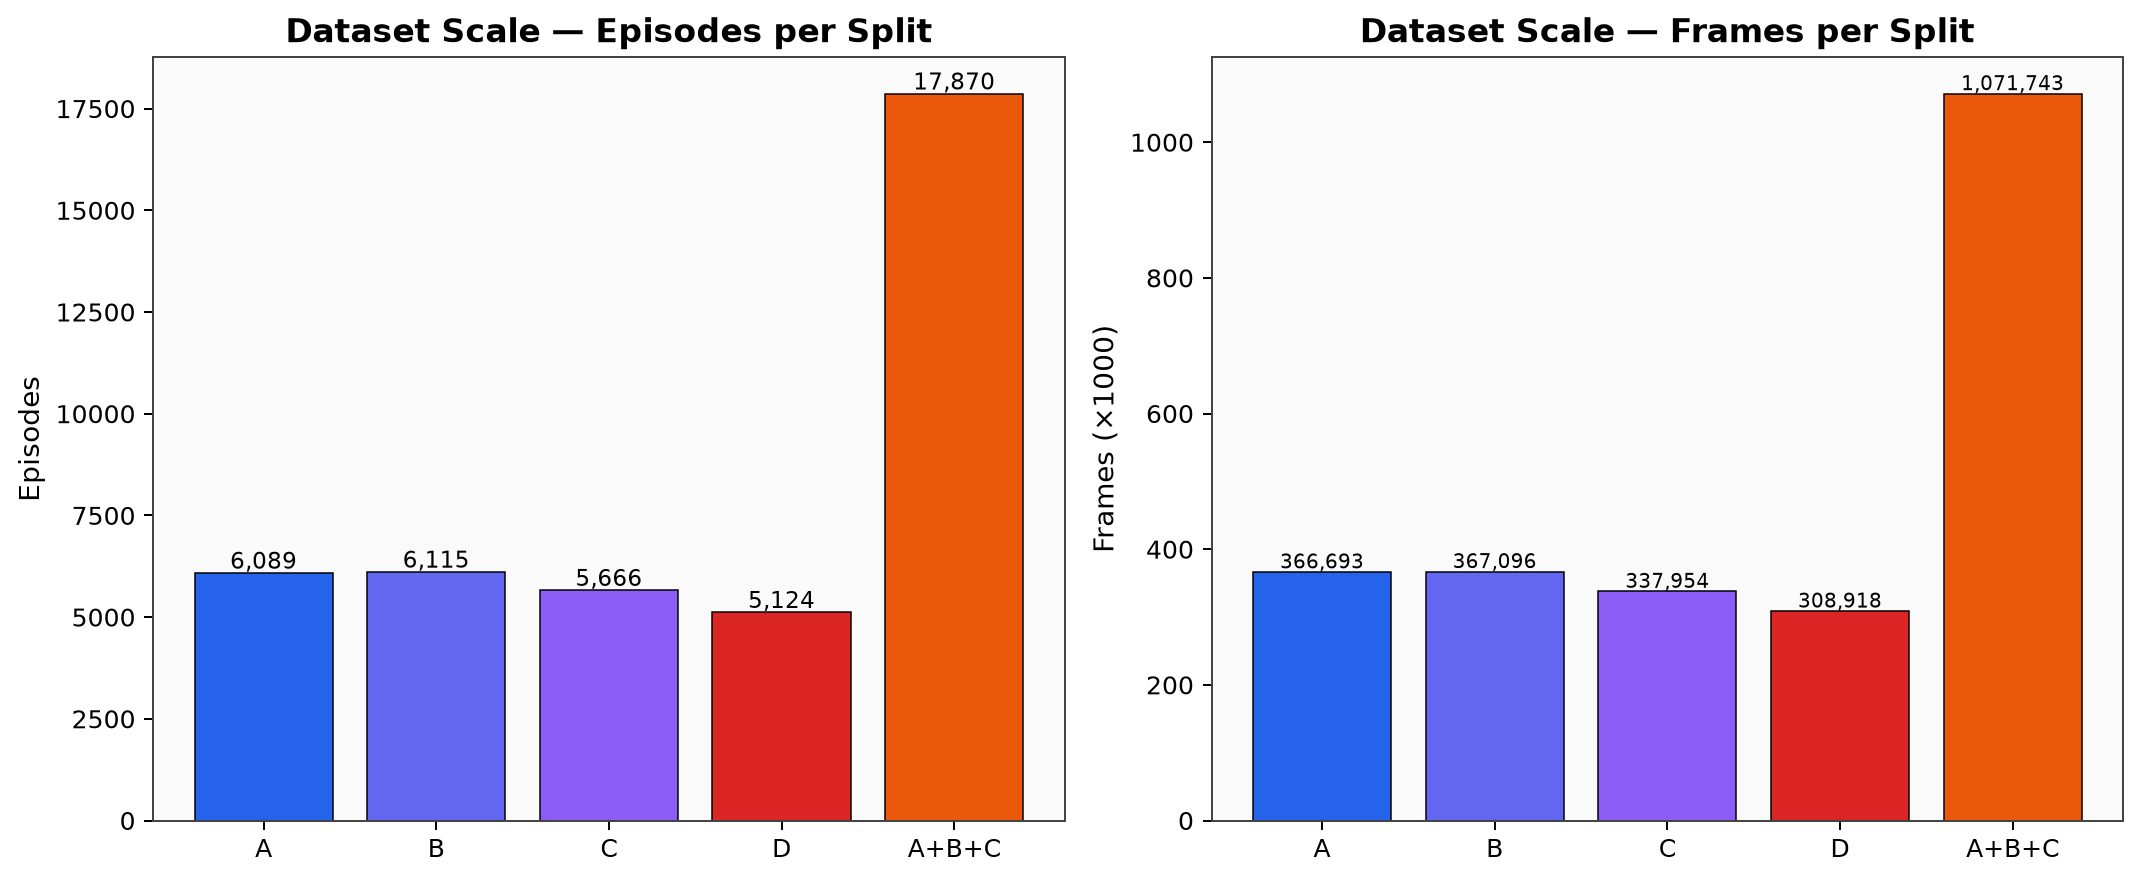
\includegraphics[width=0.88\textwidth]{dataset_scale.png}
    \caption{CALVIN 各 split 的 episode 与 frame 规模。A+B+C 合并后约为单环境数据的三倍。}
\end{figure}

数据预处理的一个关键工作是统一 LeRobot feature schema。最终采用的键名如下：

\begin{table}[H]
    \centering
    \caption{LeRobot feature schema}
    \resizebox{\textwidth}{!}{
    \begin{tabular}{lll}
        \toprule
        Key & 含义 & 备注 \\
        \midrule
        \path{observation.images.image} & 第三人称 RGB 图像 & $200\times200\times3$ \\
        \path{observation.images.wrist_image} & 腕部 RGB 图像 & $84\times84\times3$ \\
        \path{observation.state} & 机器人本体状态 & 当前帧 proprio state \\
        \path{action} & 7 维动作 & $x,y,z,roll,pitch,yaw,gripper$ \\
        \bottomrule
    \end{tabular}}
\end{table}

这个步骤不是简单改文件名，而是需要同步 parquet 列名、\path{meta/info.json}、\path{meta/stats.json} 和 per-episode stats。原因是 LeRobot 的 dataloader 只把 \path{observation.*} 前缀识别为观测，action 键也必须严格为 \path{action}。如果键名不统一，训练时会出现字段丢失或 action 不匹配。

\subsection{实验设置}

实验设置围绕训练数据域构造对照。ACT env A 模型仅使用 splitA 训练，可视为单环境 baseline；ACT A+B+C 模型使用由 splitA、splitB 和 splitC 合并得到的 merged A+B+C 数据集训练，用于评估多环境示教是否能提高未见视觉域上的泛化表现。除训练数据来源不同外，两个模型在网络结构、训练步数、batch size、随机种子、action chunk 长度和评估协议上保持一致。

\begin{table}[H]
    \centering
    \caption{对照实验设置}
    \begin{tabular}{llll}
        \toprule
        因素 & ACT env A & ACT A+B+C & 控制说明 \\
        \midrule
        训练数据 & splitA & merged A+B+C & 主要自变量 \\
        训练步数 & 1000 & 1000 & 相同快速预算 \\
        Batch size & 8 & 8 & 相同 \\
        Seed & 1000 & 1000 & 相同 \\
        Chunk size & 100 & 100 & 相同 ACT horizon \\
        评估数据 & splitD & splitD & 相同 held-out 环境 \\
        指标 & Action L1 & Action L1 & 归一化 action 空间 \\
        \bottomrule
    \end{tabular}
\end{table}

\begin{table}[H]
    \centering
    \caption{ACT 网络结构与训练超参数}
    \resizebox{\textwidth}{!}{
    \begin{tabular}{lll}
        \toprule
        类别 & 参数 & 取值 \\
        \midrule
        Policy & \path{policy.type} & act \\
        Action chunk & \path{chunk_size}, \path{n_action_steps} & 100, 100 \\
        Observation & \path{n_obs_steps} & 1 \\
        Transformer & \path{dim_model}, \path{n_heads} & 512, 8 \\
        Transformer & \path{dim_feedforward} & 3200 \\
        Transformer & \path{n_encoder_layers}, \path{n_decoder_layers} & 4, 1 \\
        VAE & \path{use_vae}, \path{latent_dim}, \path{kl_weight} & true, 32, 10.0 \\
        Vision & \path{vision_backbone} & ResNet18 \\
        Optimizer & type, learning rate, weight decay & AdamW, $1\times10^{-5}$, $1\times10^{-4}$ \\
        Training & steps, batch size, workers & 1000, 8, 4 \\
        Checkpoint & \path{save_freq} & every 500 steps \\
        Logging & WandB & offline mode \\
        \bottomrule
    \end{tabular}}
\end{table}

\subsection{训练过程}

两个模型均训练 1000 optimizer steps，并分别在 step 500 和 step 1000 保存 checkpoint。该训练预算明显小于论文级完整训练，但足以验证数据处理、策略训练和离线评估流程是否闭环，同时可以观察短训练阶段中单环境与多环境数据带来的优化差异。

\begin{figure}[H]
    \centering
    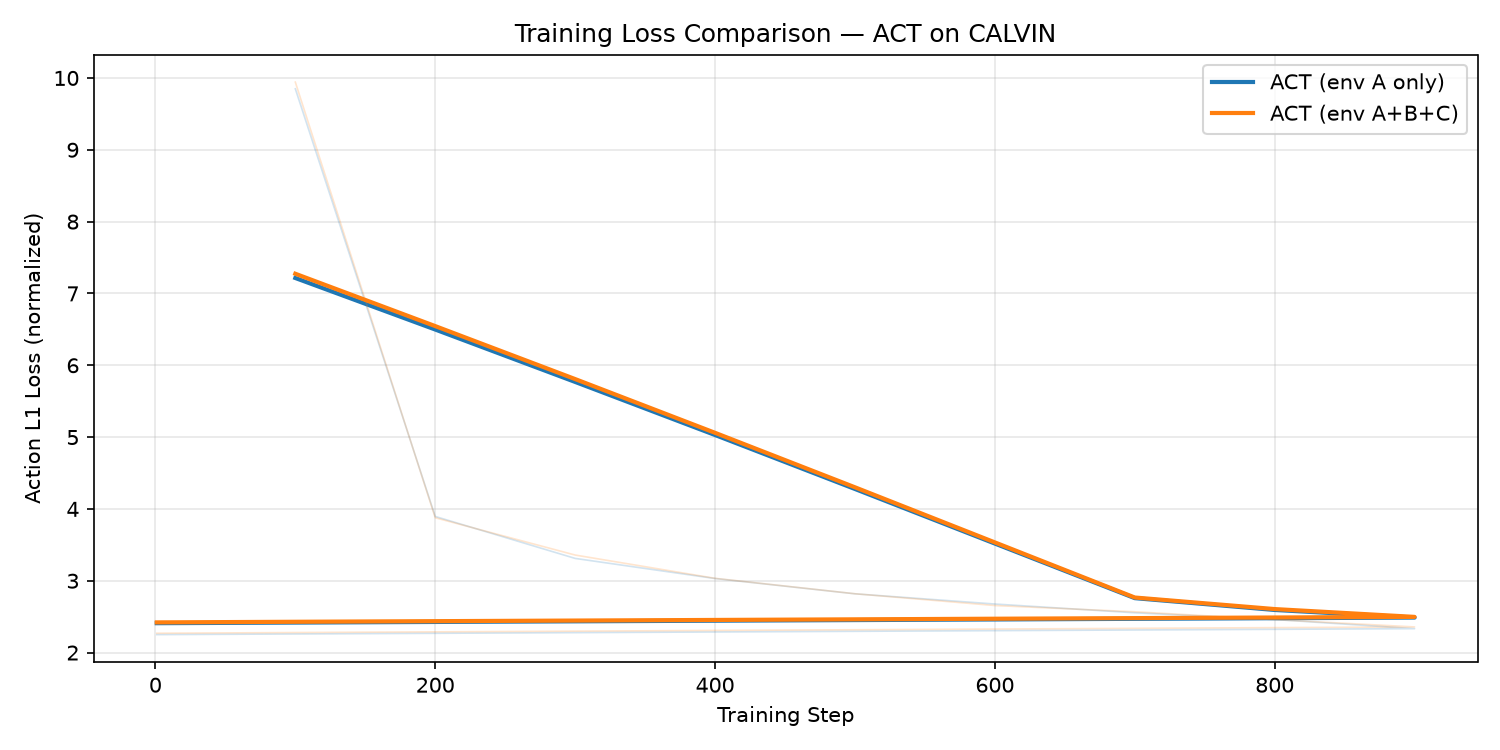
\includegraphics[width=0.82\textwidth]{training_loss_comparison.png}
    \caption{ACT env A 与 ACT A+B+C 的训练 L1 loss 曲线。两者最终训练 loss 接近。}
\end{figure}

\begin{table}[H]
    \centering
    \caption{训练阶段定量摘要}
    \resizebox{\textwidth}{!}{
    \begin{tabular}{lrrrrrrr}
        \toprule
        模型 & Step & Final loss & Grad norm & Data s & Smp/s & Train wall & Total wall \\
        \midrule
        ACT env A & 1000 & 2.250 & 62.439 & 0.444 & 15 & 543s & 545s \\
        ACT A+B+C & 1000 & 2.269 & 62.254 & 0.572 & 12 & 711s & 1472s \\
        \bottomrule
    \end{tabular}}
\end{table}

可以看到，两模型训练 loss 从约 10 降到约 2.2，说明 ACT 已经学到基本 action 映射，但仍未完全收敛。多环境模型最终 loss 只比单环境模型高 0.019，训练侧差异并不大。真正显著的工程差异来自数据加载：merged A+B+C 数据集包含 17870 episodes 和 1071743 frames，构建索引与采样开销明显高于单 split。

\begin{figure}[H]
    \centering
    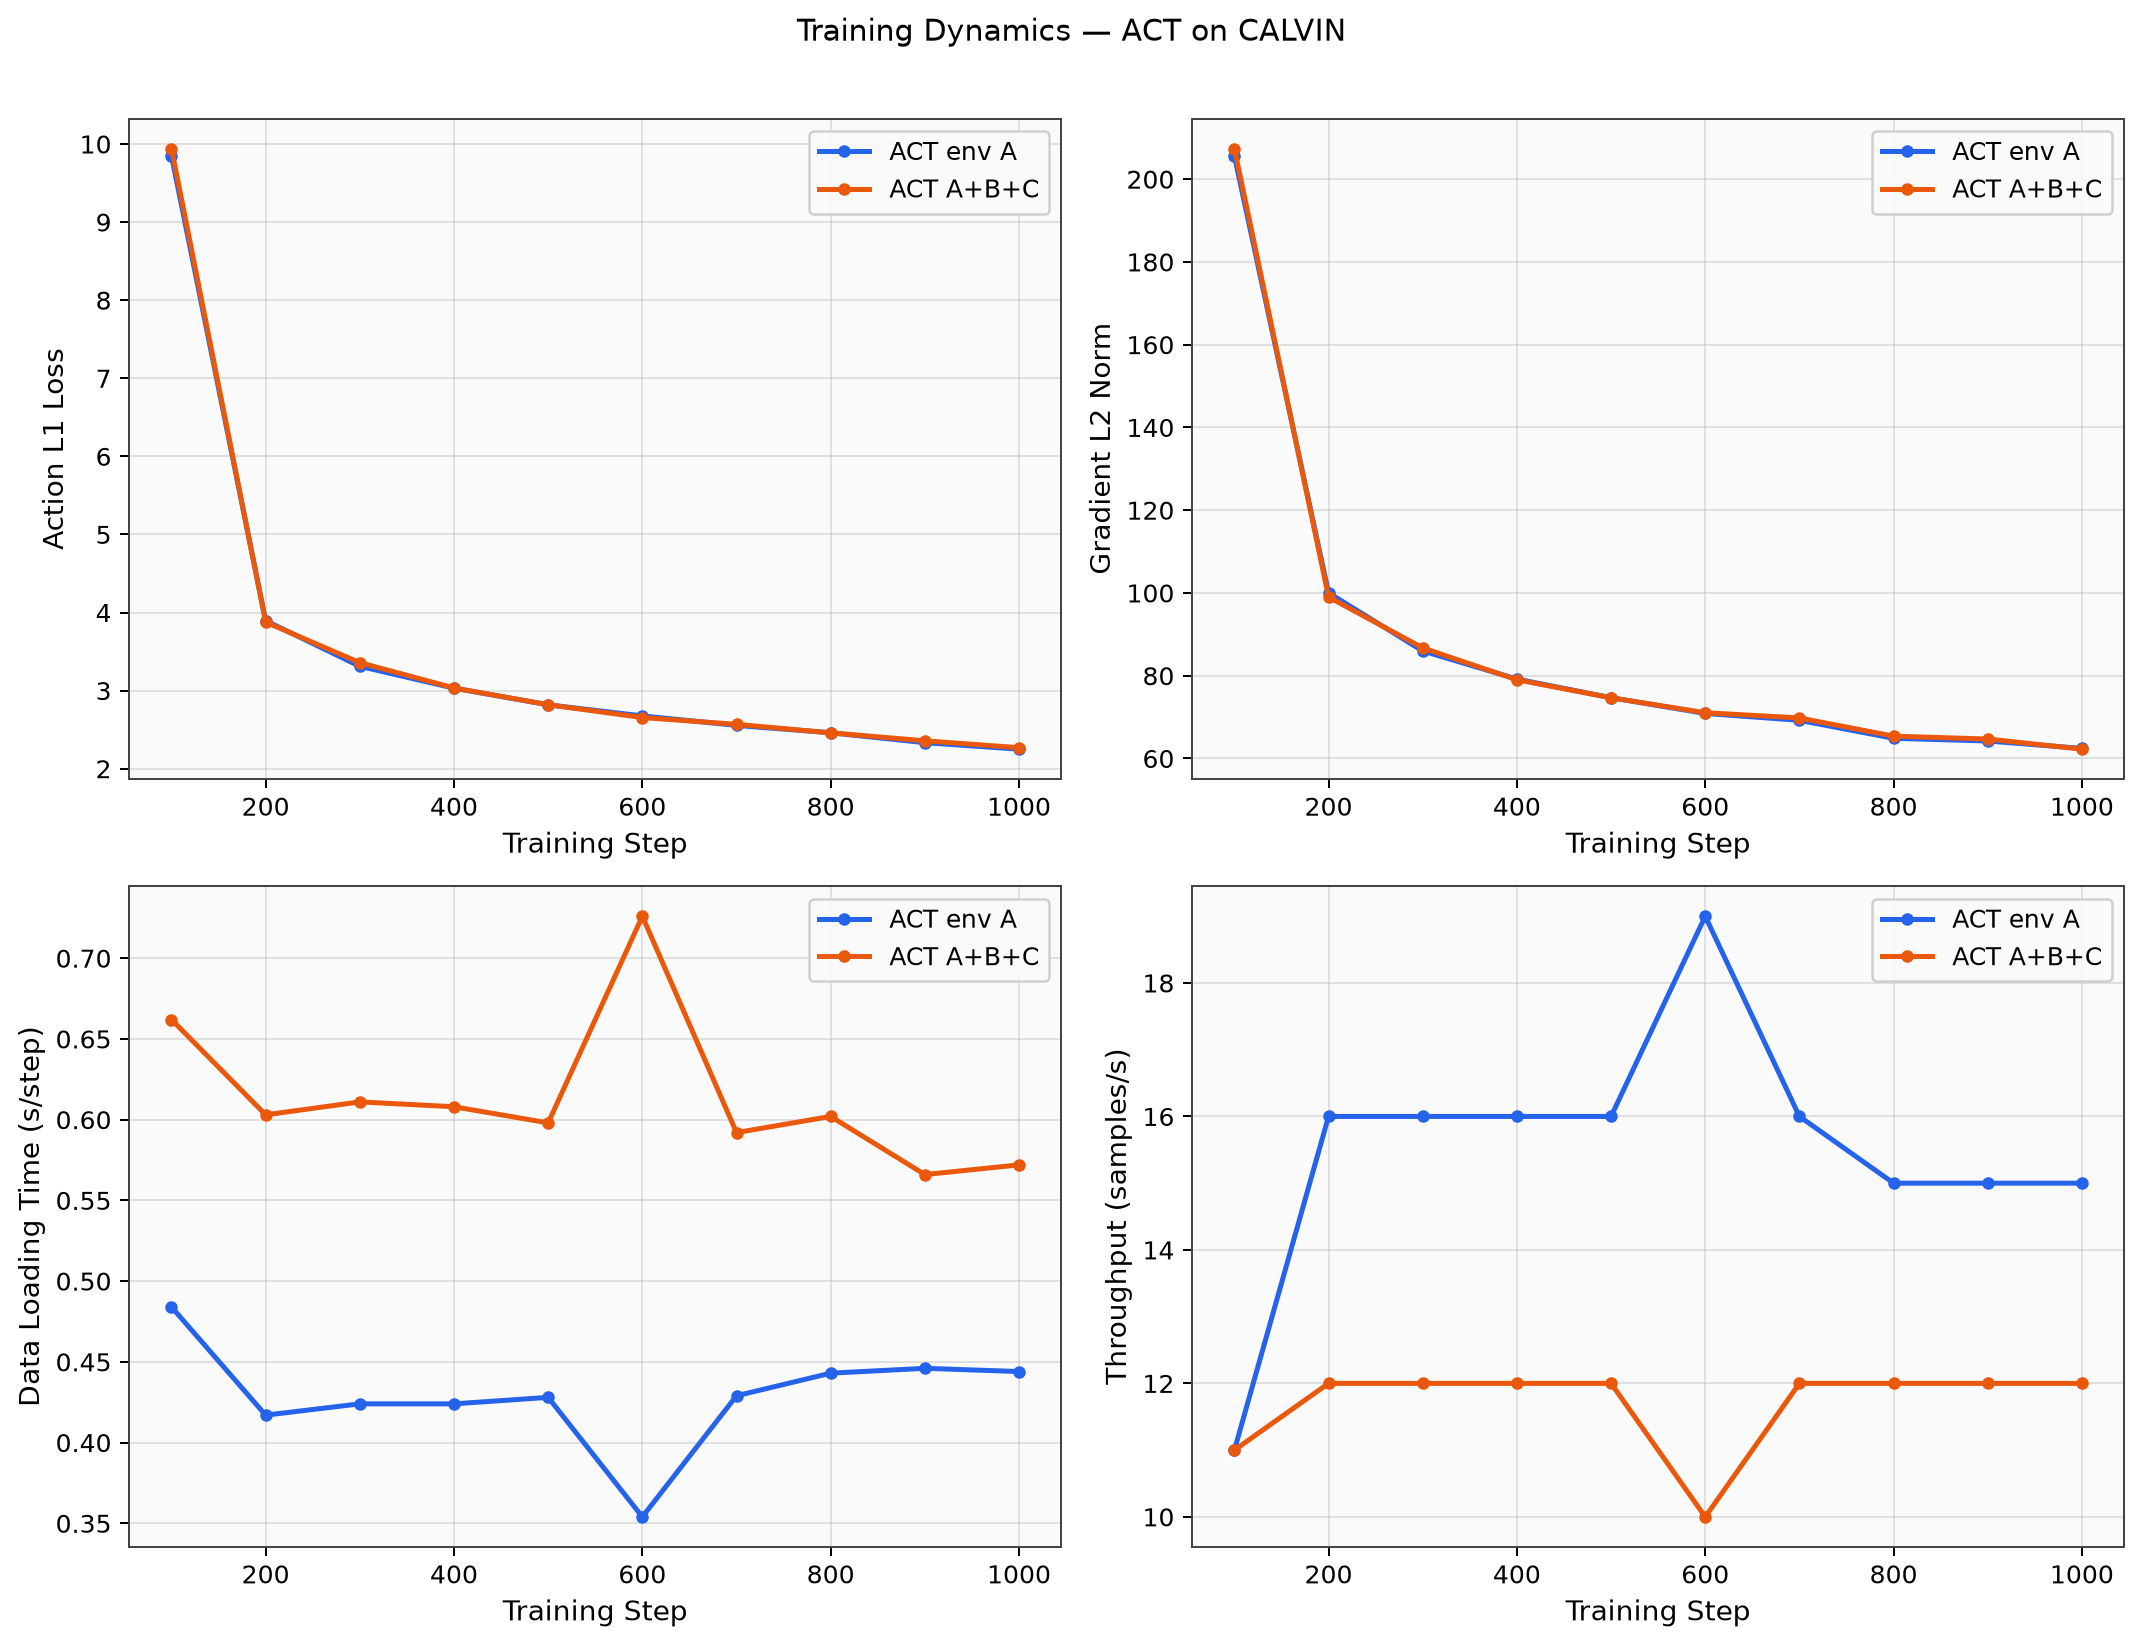
\includegraphics[width=0.95\textwidth]{training_dashboard.png}
    \caption{训练动态：loss、梯度范数、数据加载时间和吞吐。A+B+C 的数据加载成本明显更高。}
\end{figure}

\subsection{零样本泛化结果}

评估时，模型输入 splitD 的当前第三人称图像、腕部图像和机器人状态，输出长度 100 的 action chunk。本报告主指标比较 chunk index 0 的预测动作与 ground truth action 的平均 L1 误差。所有 L1 均在归一化 action 空间中计算。

\begin{table}[H]
    \centering
    \caption{环境 D zero-shot Action L1 结果}
    \begin{tabular}{llrrrr}
        \toprule
        Eval 设置 & 模型 & Samples & Mean L1 $\downarrow$ & Std L1 & Wall \\
        \midrule
        快速 eval & ACT env A & 320 & \textbf{0.679} & 0.644 & 94s \\
        快速 eval & ACT A+B+C & 320 & 0.745 & 0.655 & 89s \\
        中等 eval & ACT env A & 400 & \textbf{0.687} & 0.639 & 124s \\
        中等 eval & ACT A+B+C & 400 & 0.764 & 0.650 & 115s \\
        \bottomrule
    \end{tabular}
\end{table}

\begin{figure}[H]
    \centering
    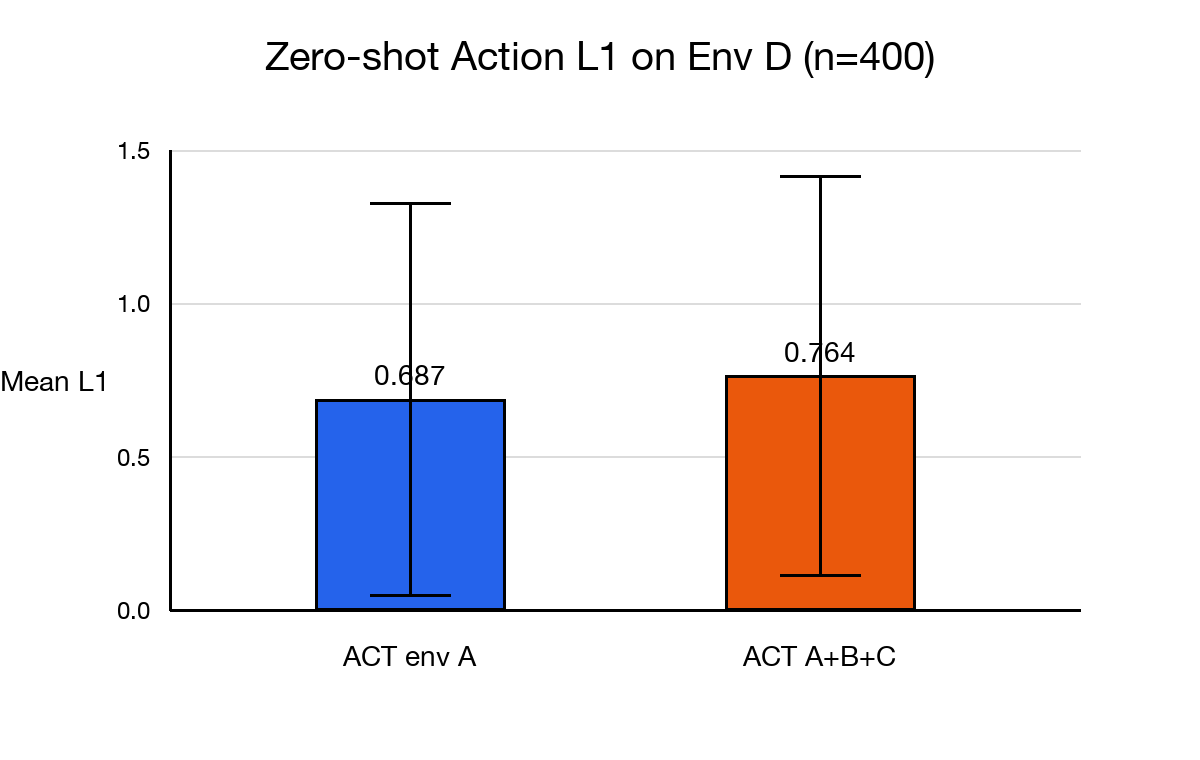
\includegraphics[width=0.70\textwidth]{eval_medium_overall_report.png}
    \caption{中等规模 eval 的 D 域 zero-shot Mean L1。短训练预算下，env A baseline 低于 A+B+C。}
\end{figure}

快速 eval 与中等 eval 的趋势一致：在 1000-step 快速预算下，单环境 env A 模型在未见环境 D 上的 Action L1 反而低于 A+B+C 模型。中等 eval 中，A+B+C 的 Mean L1 比 env A 高约 11.2\%。这不说明多环境训练无效，更合理的解释是：1000 steps 对 107 万帧 merged 数据过短，多环境模型还没有充分从多域多样性中受益。

\begin{table}[H]
    \centering
    \caption{中等 eval 的分维度 Mean L1}
    \resizebox{\textwidth}{!}{
    \begin{tabular}{lrrrrrrrr}
        \toprule
        模型 & Overall & x & y & z & roll & pitch & yaw & gripper \\
        \midrule
        ACT env A & \textbf{0.687} & \textbf{0.838} & \textbf{0.579} & 0.834 & \textbf{0.686} & \textbf{0.851} & \textbf{0.479} & \textbf{0.540} \\
        ACT A+B+C & 0.764 & 0.953 & 0.661 & \textbf{0.802} & 0.695 & 0.892 & 0.523 & 0.819 \\
        $\Delta$ ABC-A & +0.077 & +0.115 & +0.082 & -0.032 & +0.009 & +0.041 & +0.045 & +0.280 \\
        \bottomrule
    \end{tabular}}
\end{table}

\begin{figure}[H]
    \centering
    \begin{subfigure}[b]{0.49\textwidth}
        \centering
        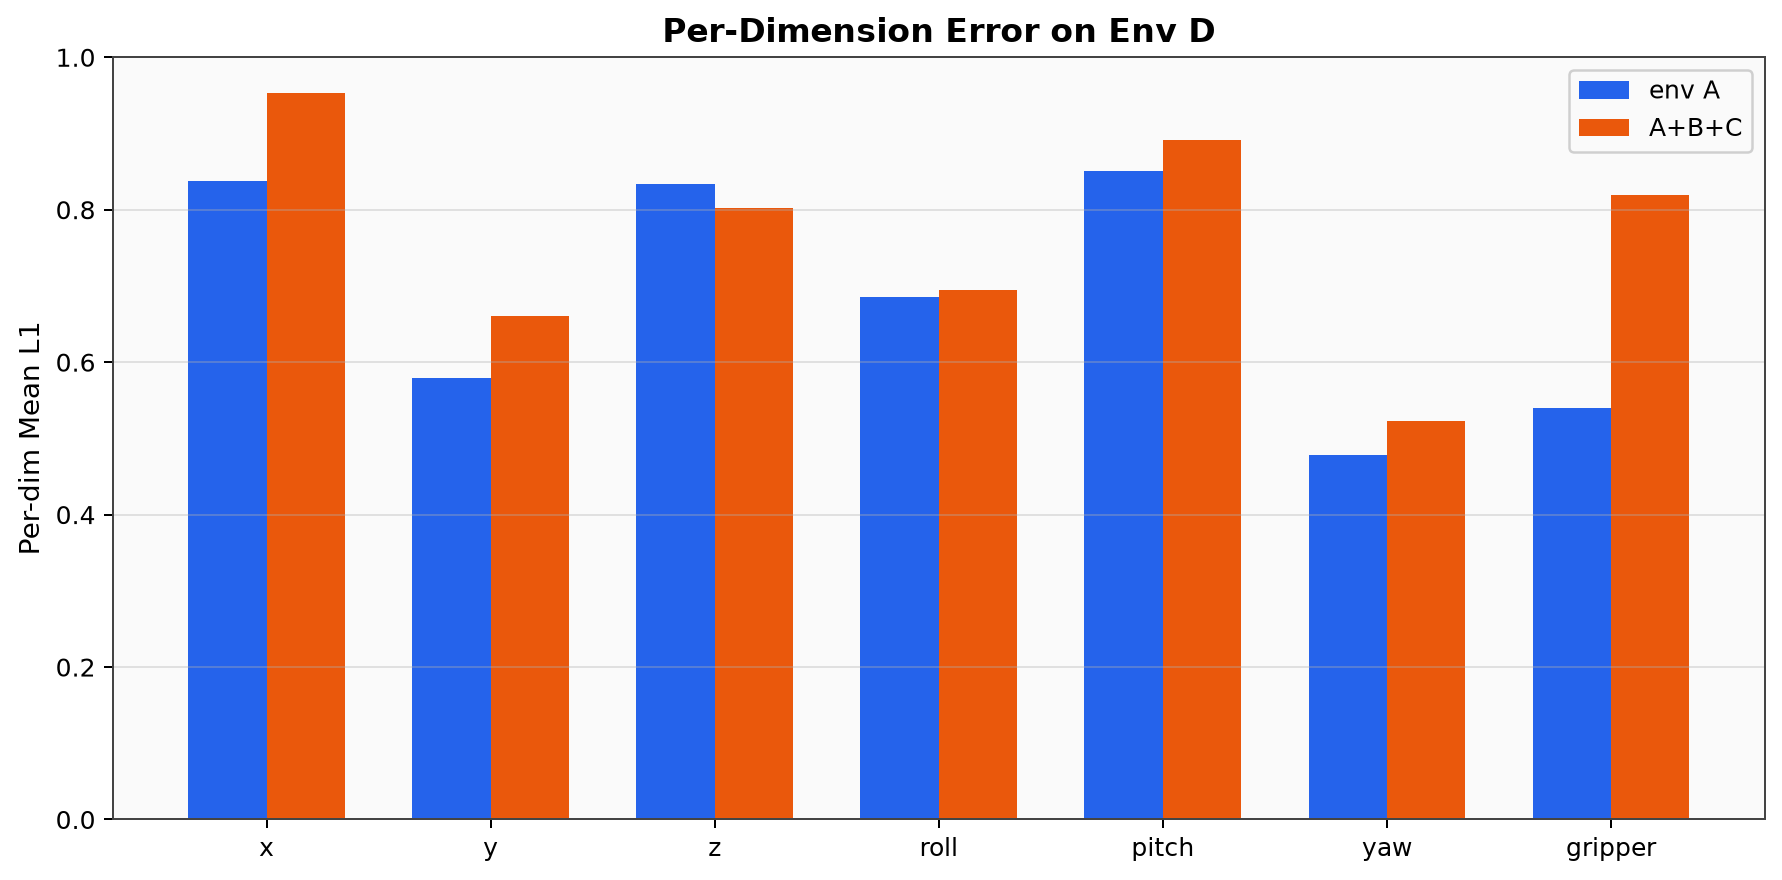
\includegraphics[width=\textwidth]{eval_medium_per_dim.png}
        \caption{分维度 L1 对比}
    \end{subfigure}
    \hfill
    \begin{subfigure}[b]{0.49\textwidth}
        \centering
        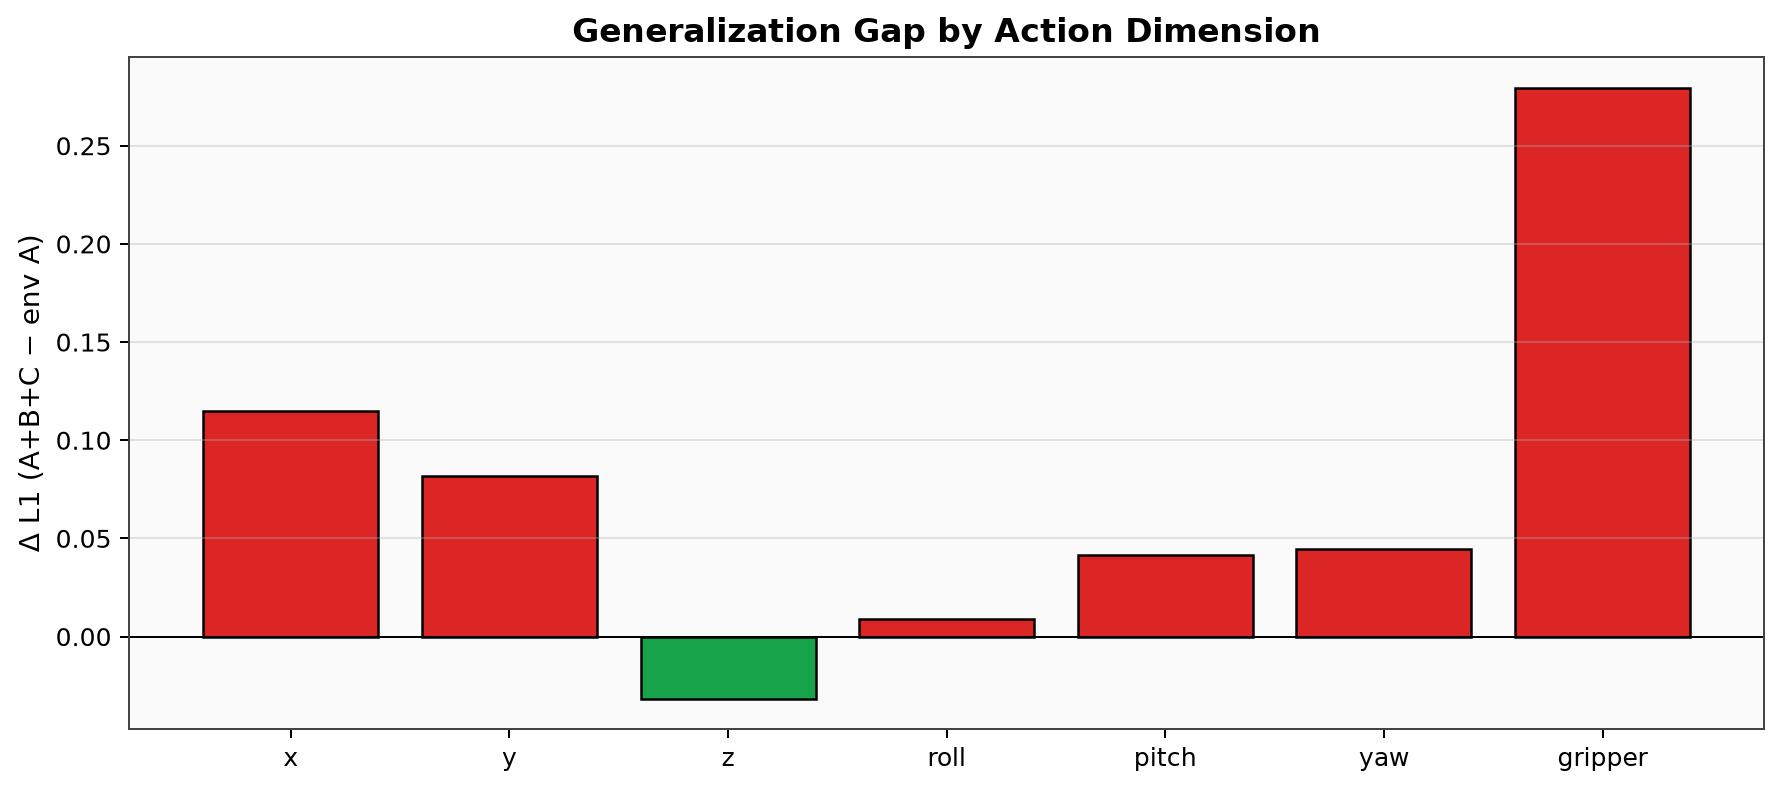
\includegraphics[width=\textwidth]{eval_delta_per_dim.png}
        \caption{A+B+C 相对 env A 的差值}
    \end{subfigure}
    \caption{分维度泛化误差。A+B+C 仅在 z 维略优，gripper 维度差距最大。}
\end{figure}

分维度结果显示，env A baseline 在 6/7 个动作维度上误差更低，多环境模型仅在 z 维略优。差距最大的维度是 gripper，说明短训练下模型对夹爪开合相关视觉语义的跨环境对齐还不充分。

\begin{figure}[H]
    \centering
    \begin{subfigure}[b]{0.49\textwidth}
        \centering
        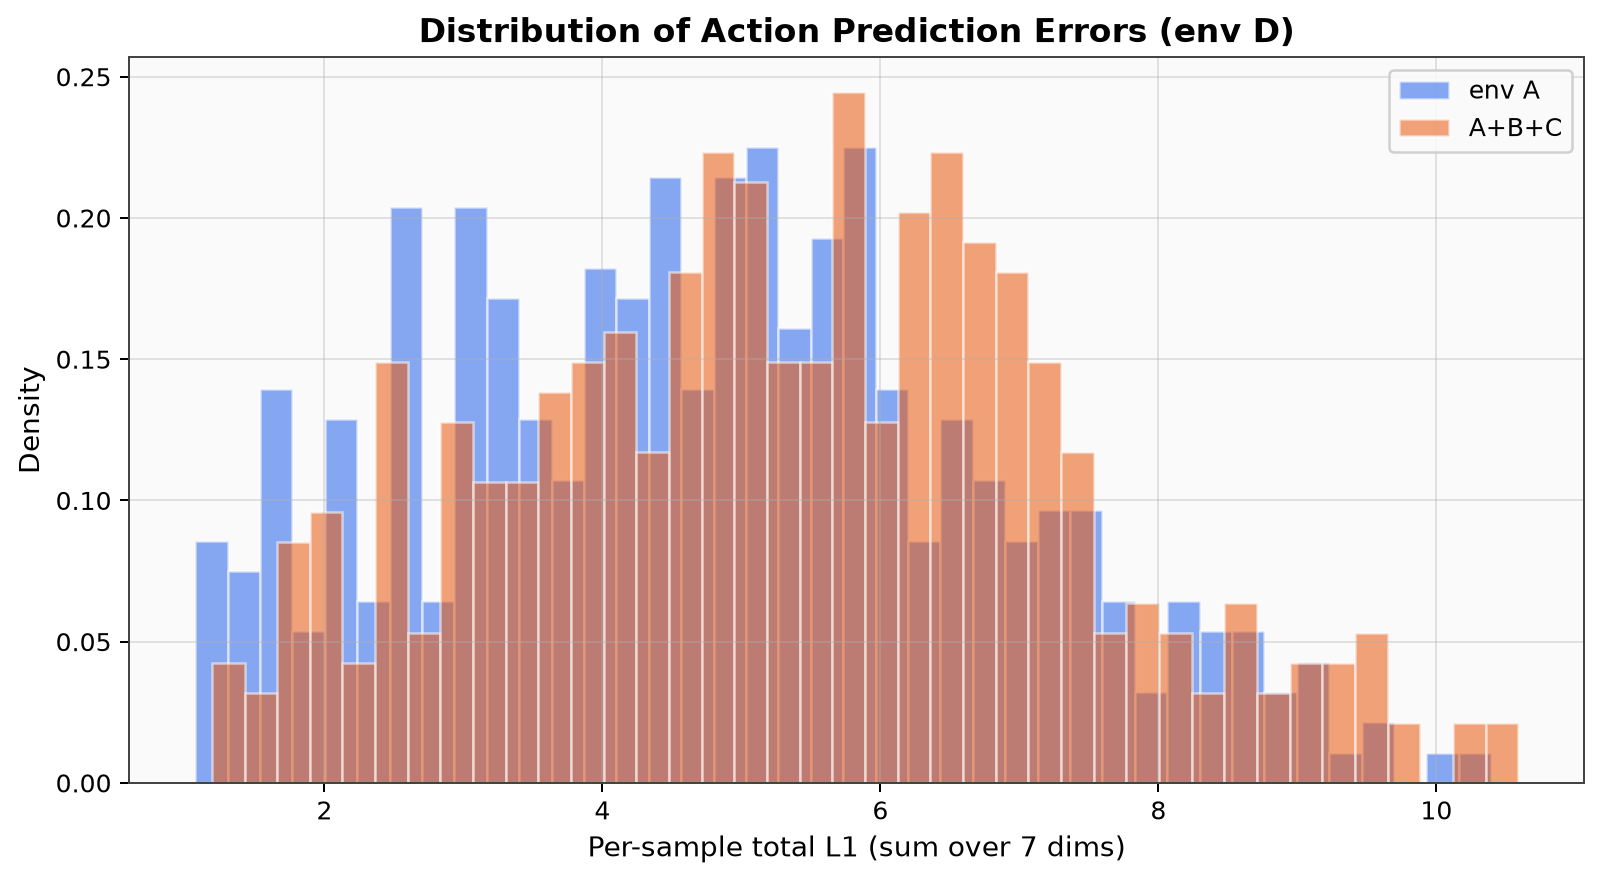
\includegraphics[width=\textwidth]{eval_error_histogram.png}
        \caption{样本总 L1 直方图}
    \end{subfigure}
    \hfill
    \begin{subfigure}[b]{0.49\textwidth}
        \centering
        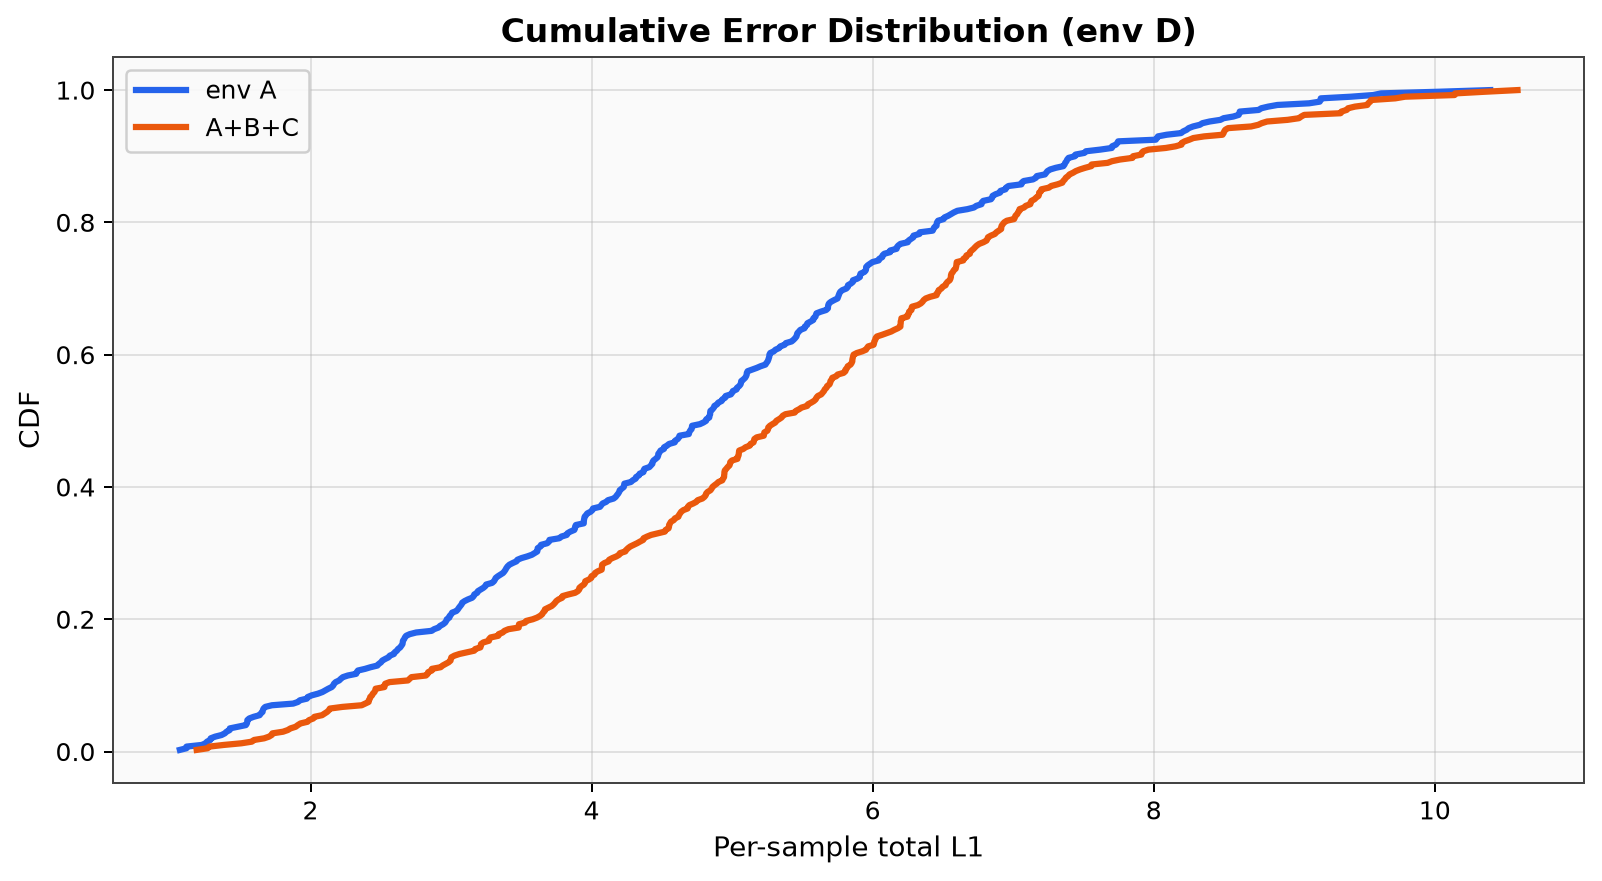
\includegraphics[width=\textwidth]{eval_error_cdf.png}
        \caption{样本总 L1 CDF}
    \end{subfigure}
    \caption{误差分布与 CDF，用于观察 tail error，而不仅仅依赖均值。}
\end{figure}

\subsection{补充分析}

除主评估外，实验进一步分析了训练步数和 action chunk horizon 对结果的影响。checkpoint 消融用于判断 1000 steps 是否已经接近泛化饱和；chunk horizon 分析则用于观察 ACT 一次预测 100 步动作时，不同时间位置的误差变化。

\begin{table}[H]
    \centering
    \caption{env A checkpoint 消融}
    \begin{tabular}{lrrr}
        \toprule
        Checkpoint & Samples & Mean L1 $\downarrow$ & Wall \\
        \midrule
        step 500 & 320 & 0.731 & 100.8s \\
        step 1000 & 320 & \textbf{0.679} & 89.3s \\
        \bottomrule
    \end{tabular}
\end{table}

\begin{figure}[H]
    \centering
    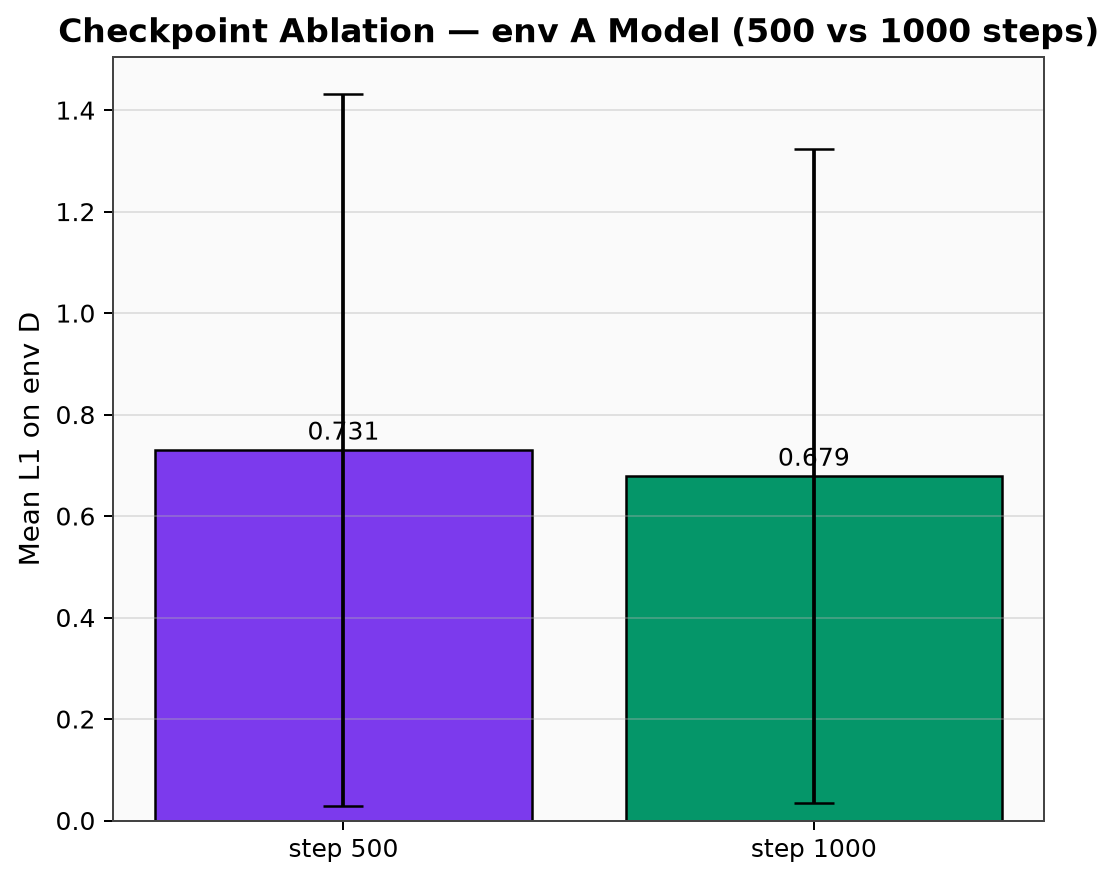
\includegraphics[width=0.62\textwidth]{ablation_checkpoint_envA.png}
    \caption{step 500 与 step 1000 checkpoint 在 D 域上的 Action L1。继续训练仍有收益。}
\end{figure}

从 500 到 1000 steps，Mean L1 从 0.731 降至 0.679，下降约 7.1\%。这说明 1000 steps 仍远未泛化饱和，若继续训练到 50k steps 或更长，结果可能发生变化。

\begin{table}[H]
    \centering
    \caption{不同 chunk index 的 D 域 Mean L1}
    \begin{tabular}{lrrrrrrr}
        \toprule
        模型 & 0 & 1 & 5 & 10 & 25 & 50 & 99 \\
        \midrule
        ACT env A & 0.681 & 0.686 & 0.674 & 0.690 & 0.686 & 0.678 & 0.784 \\
        ACT A+B+C & 0.735 & 0.732 & 0.719 & 0.722 & 0.698 & 0.675 & 0.814 \\
        \bottomrule
    \end{tabular}
\end{table}

\begin{figure}[H]
    \centering
    \begin{subfigure}[b]{0.58\textwidth}
        \centering
        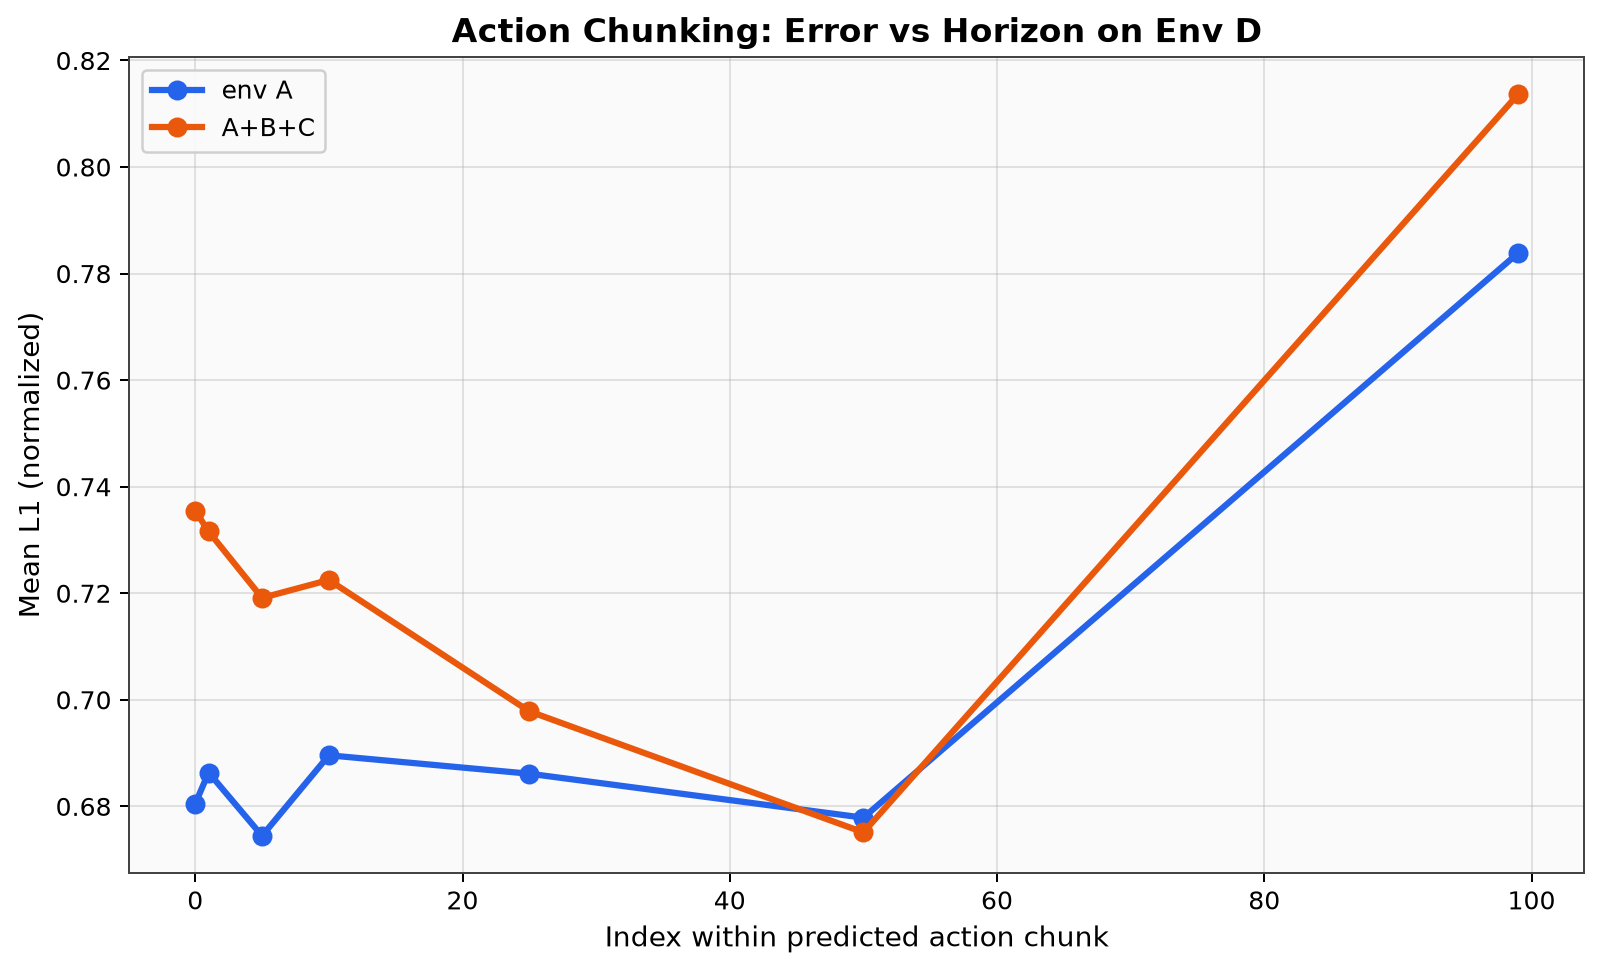
\includegraphics[width=\textwidth]{chunk_horizon_l1.png}
        \caption{chunk 内不同 horizon 的 L1 曲线}
    \end{subfigure}
    \hfill
    \begin{subfigure}[b]{0.38\textwidth}
        \centering
        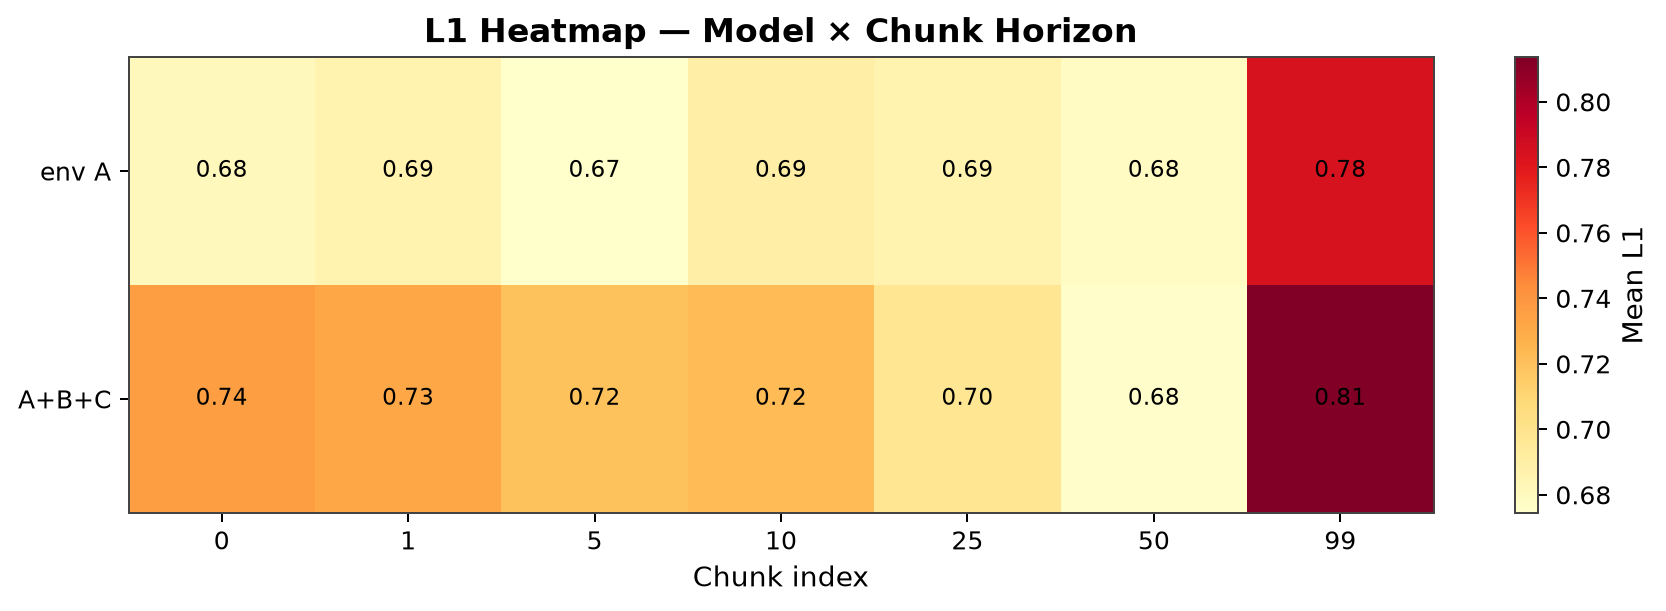
\includegraphics[width=\textwidth]{chunk_horizon_heatmap.png}
        \caption{模型与 chunk index 热力图}
    \end{subfigure}
    \caption{Action chunk horizon 分析。index 99 处误差明显上升，说明部署时应采用 receding horizon。}
\end{figure}

env A 从 index 0 到 99 的 L1 增长约 15.2\%，A+B+C 增长约 10.7\%。因此，虽然 ACT 一次输出 100 步动作，但实际部署时不适合直接执行 100 步开环动作，更合理的方式是每一步或每隔若干步重新调用策略更新 chunk。

\subsection{耗时统计}

\begin{figure}[H]
    \centering
    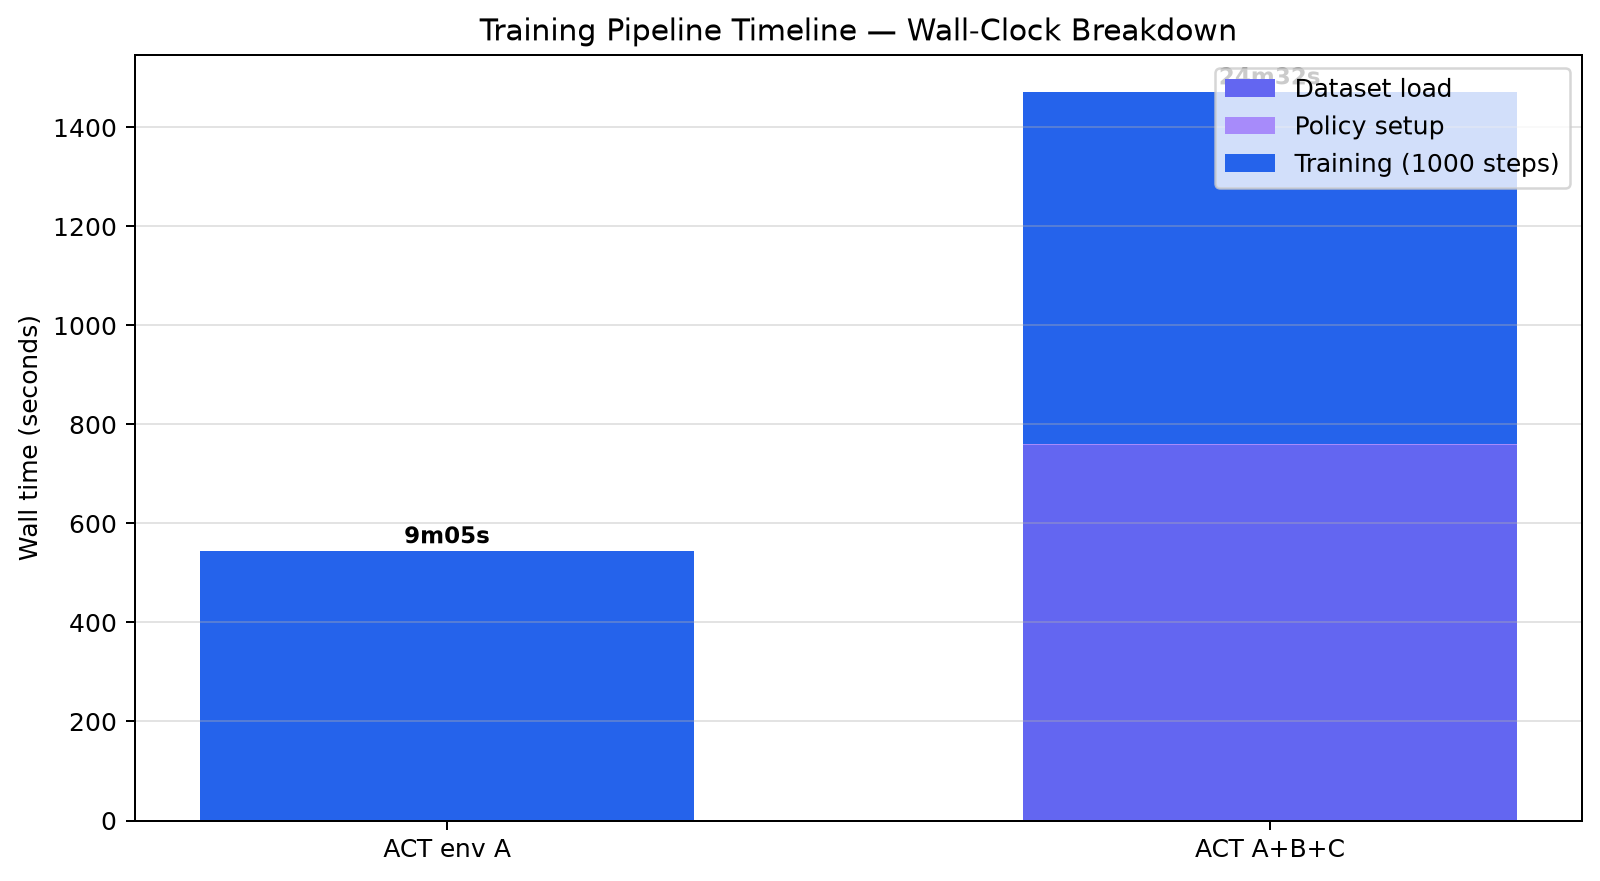
\includegraphics[width=0.78\textwidth]{timing_training_timeline.png}
    \caption{训练 pipeline wall-clock 分解。多环境模型的额外成本主要来自 merged 数据集加载。}
\end{figure}

\begin{table}[H]
    \centering
    \caption{题目二训练与评估耗时}
    \begin{tabular}{lrrl}
        \toprule
        阶段 & ACT env A & ACT A+B+C & 说明 \\
        \midrule
        数据集加载 & 0s & 759s & merged 数据集索引构建较慢 \\
        策略初始化 & 2s & 2s & 基本一致 \\
        训练 1000 steps & 543s & 711s & A+B+C 每 step 更慢 \\
        训练总 wall & 545s & 1472s & A+B+C 约 24m32s \\
        快速 eval & 94s & 89s & 320 samples/model \\
        中等 eval & 124s & 115s & 400 samples/model \\
        补充实验总 wall & \multicolumn{2}{c}{609s} & checkpoint + chunk + 分布 \\
        \bottomrule
    \end{tabular}
\end{table}

从耗时统计可以看出，多环境训练的主要额外成本并不只来自反向传播本身，也来自 merged 数据集的索引构建和采样开销。若后续将训练扩展到 50k steps 或更长，应优先考虑数据缓存、shard 组织和本地 SSD 读取，否则 A+B+C 训练会在大规模实验中形成明显瓶颈。

\subsection{讨论与局限}

本实验的主要现象是：在 1000-step 快速预算下，ACT env A 在环境 D 上的 Action L1 低于 ACT A+B+C。这个结果不能简单解释为“多环境训练无效”。更合理的判断是，多环境模型面对更宽的数据分布，需要更长训练才能学到跨域不变特征；当前 1000 steps 对 A+B+C 的 107 万帧数据只覆盖很小比例，明显处于欠训练状态。

本实验仍存在若干局限。首先，实验没有部署 CALVIN 官方仿真环境，因此无法报告长任务 Success Rate，只能使用离线 Action L1 衡量模仿质量。其次，1000 steps 属于快速验证预算，两个模型都没有充分收敛，尤其是 A+B+C 模型面对更大的训练集时欠训练更明显。此外，环境 D 的评估采用子采样方式，且实验只运行单个随机种子，因此结果应被视为趋势性观察，而不是具有统计置信区间的最终结论。最后，不同训练集和评估集的归一化统计也可能引入轻微不可比因素。

总体而言，本实验完成了 LeRobot ACT 跨环境泛化的主要实验闭环。结果显示，在短训练预算下，多环境数据并没有立即转化为更低的 D 域 Action L1；但 checkpoint 消融和训练曲线也表明模型仍处于继续改进阶段。后续若要得到更强结论，需要进行更长训练、多随机种子实验、全量或更大规模 D 域评估，并补充 CALVIN 仿真 success rate。

\section{补充材料}

\subsection{GitHub 仓库}

代码与轻量交付材料已整理到 GitHub 仓库，完整链接如下：
\begin{center}
{\small \url{https://github.com/Boringredduck/hw3}}
\end{center}

题目一材料位于 \path{docs/experiment1_3d_assets/}。其中，\path{images/} 保存输入图、重建结果和生成结果截图；\path{models/} 保存扑克牌、鼠标、充电插头和 garden 场景的 OBJ/PLY 交付模型；\path{videos/} 保存单物体环绕视频和 Blender 最终融合渲染视频。

题目二代码和材料分开整理。可运行脚本位于仓库根目录的 \path{scripts/}，包括数据下载、数据预处理、ACT 训练、环境 D 测试和结果绘图入口；实验文档、图表和统计结果位于 \path{docs/experiment2_act/}，其中 \path{figures/} 保存训练曲线和评估图，\path{stats/} 保存数据规模、训练耗时和评估统计表，\path{results/} 保存小型评估 JSON。最终报告 PDF、LaTeX 源文件和报告图片位于 \path{docs/final_report/}。

仓库未提交 CALVIN 训练/验证/测试数据、ACT checkpoint、模型权重、wandb 日志和本地训练输出目录，以避免 GitHub 仓库体积过大。

\subsection{模型权重与完整实验结果}

模型权重和完整实验结果通过百度网盘分享，文件名为“实验结果与模型权重”。完整链接如下：
\begin{center}
{\small \url{https://pan.baidu.com/s/1Vxqe9ldj-p4FHISICwnSig}}
\end{center}
提取码：\texttt{mfkd}。

\section{总结与展望}

本报告围绕空间智能中的场景建模与策略泛化两个层面完成实验。题目一从真实多视角重建、文本到 3D、单图到 3D 和背景 3DGS 重建出发，将多个来源的资产统一到 Blender 中完成融合渲染，验证了多源 3D 内容生成与真实场景组合的基本流程。实验结果表明，3DGS 在具有足够视角覆盖和稳定纹理的目标上能够恢复较清晰的几何结构，但对阴影、背景粘连、植被等复杂区域仍较敏感；AIGC 生成方法能够快速得到语义上合理的物体外观，但精细几何和不可见区域推断仍存在不稳定性。

题目二基于 LeRobot 实现了 CALVIN 数据整理、ACT 策略训练和环境 D zero-shot 离线评估。实验通过 env A 单环境模型和 A+B+C 多环境模型构造对照，比较了两种训练数据设置在未见环境上的 action prediction 误差。结果显示，在 1000-step 快速训练预算下，多环境训练并没有立即带来更低的 D 域 Action L1；结合 checkpoint 消融、chunk horizon 分析和训练耗时统计可以看出，A+B+C 模型面对更大的数据分布时仍明显欠训练，当前结果更适合作为完整实验流程的验证和趋势性观察，而不是对多环境泛化能力的最终定论。

后续工作可以从三个方向继续改进。首先，题目一可补充更稳定的拍摄流程、前景分割和尺度标定，并在融合阶段加入更一致的光照估计与材质调整，以提升多资产场景的一致性。其次，题目二应扩展到更长训练步数、多随机种子和更大规模环境 D 评估，并尽可能接入 CALVIN 官方仿真环境报告 Success Rate。最后，可以进一步比较 ACT 与 Diffusion Policy 等策略模型在相同数据设置下的泛化差异，从而更系统地分析视觉域变化、数据规模和动作建模方式对具身智能策略学习的影响。

\end{document}
